\documentclass[10pt]{article}

\usepackage[a4paper,hmargin=1.5cm,vmargin=2cm]{geometry}
%\setlength{\columnsep}{0.7cm}
\usepackage{amsmath}
\usepackage{graphicx}
\usepackage{caption}
\usepackage{balance}
\usepackage[varqu]{inconsolata}

\usepackage[utf8]{inputenc}
\usepackage[super,sort]{natbib}
\bibliographystyle{unsrtnat}
\setlength{\bibsep}{0.3ex plus 0.2ex}
\usepackage[dvipsnames]{xcolor}
\usepackage[compact]{titlesec}
\usepackage[hypertexnames=false]{hyperref}
\hypersetup{
    colorlinks,
    linkcolor={blue!50!black},
    citecolor={blue!50!black},
    urlcolor={blue!50!black}
}
\urlstyle{same} % no tt font for URLs
\renewcommand{\topfraction}{0.9}
\renewcommand{\dbltopfraction}{0.9}
\renewcommand{\textfraction}{0.1}
\clubpenalty=1000
\widowpenalty=1000
\displaywidowpenalty=1000



\begin{document}

{\centering\phantomsection\addcontentsline{toc}{section}{Title}
\textbf{\Large Analyzing single-cell bisulfite sequencing data with \textit{MethSCAn}}\\[1.5ex]

Lukas P.~M. Kremer\textsuperscript{1,2,*},
Martina M. Braun\textsuperscript{2},
Svetlana Ovchinnikova\textsuperscript{1},
Leonie Küchenhoff\textsuperscript{1,2},\\
Santiago Cerrizuela\textsuperscript{2},
Ana Martin-Villalba\textsuperscript{2,*},
Simon Anders\textsuperscript{1,*}\\[2em]
}
\noindent\textsuperscript{1} BioQuant Centre, University of Heidelberg, Heidelberg, Germany\\
\textsuperscript{2} Division of Molecular Neurobiology, German Cancer Research Center (DKFZ), Heidelberg, Germany\\
\textsuperscript{*} corresponding authors. e-mails:\\
\texttt{l.kremer@dkfz-heidelberg.de}\\
\texttt{a.martin-villalba@dkfz-heidelberg.de}\\
\texttt{simon.anders@bioquant.uni-heidelberg.de}


\section*{Abstract}

\noindent Single-cell bisulfite sequencing (scBS) is a technique that enables the assessment of DNA methylation at single-base pair and single-cell resolution.
The analysis of large datasets obtained from scBS requires preprocessing to reduce data size, improve signal-to-noise ratio, and provide interpretability.
Typically, this is achieved by dividing the genome into large tiles and averaging the methylation signals within each tile.

Here, we demonstrate that this coarse-graining approach can lead to signal dilution.
We propose improved strategies to identify more informative regions for methylation quantification, and a more accurate quantitation method than simple averaging.
Our approach enables better discrimination of cell types and other features of interest and reduces the need for large numbers of cells.
We also present an approach to detect differentially methylated regions (DMRs) between groups of cells, and demonstrate its ability to identify biologically meaningful regions that are associated with genes involved in the core functions of specific cell types.

Finally, we present the software tool \textit{MethSCAn} for scBS data analysis: \url{https://anders-biostat.github.io/MethSCAn}


\section*{Main Text}
\section*{Introduction}

Sequencing-based assays with single-cell resolution have offered new means to understand the differences between the cells making up a sample.
Single-cell RNA sequencing (scRNA-seq) techniques have matured at great pace in recent years, with well developed analysis methodology, and methods to study epigenetics at single-cell resolution are rapidly catching up.


Briefly, in a bisulfite sequencing assay DNA is treated with bisulfite, which converts unmethylated cytosines to uracils which are read as thymine in subsequent PCR, while methylated cytosines are protected from conversion.
After sequencing, these conversions allow for the determination of the methylation status of all cytosines covered by reads \citep{Frommer_1992}.
Bisulfite sequencing can also be performed at single-cell resolution \citep{Smallwood_2014} and even in parallel with scRNA-seq \citep{scMTseq,Clark2018}.

In the present paper, we discuss strategies to analyze single-cell bisulfite-sequencing (scBS) data.
We suggest improvements to current approaches, and demonstrate their value in benchmarks, using four real-world datasets.
Furthermore, we discuss how to perform comparative analyses.
Finally, we present \textit{MethSCAn}, a comprehensive software toolkit to perform scBS data analysis.



The standard approach to analyze scBS data is based on methodology developed for the analysis of scRNA-seq data.
Therefore, we start by briefly reviewing how sc\emph{RNA}-seq data is commonly analyzed, before we discuss scBS data analysis.

The starting point in most scRNA-seq analyses is a matrix of UMI counts (i.e.\ counts of distinct RNA molecules), one row for each cell and one column for each gene.
A first goal is usually to assign cell types or states to cells.
To this end, one needs to establish which cells are similar to each other, i.e., quantify the distance (i.e., dissimilarity) between any two given cells' transcriptional profile.
A standard approach, used with minor variation in virtually all recent research and automated by popular software such as Seurat \citep{seurat5} or Scanpy \citep{Wolf_2018}, is as follows:
One first accounts for cell-to-cell variation in sequencing depth by dividing each UMI count by the respective cell's total UMI count, then transforms to a homoskedastic scale by taking the logarithm.
In order to avoid matrix elements with zero count to be transformed to minus infinity, one typically adds a very small ``pseudocount'' (often $10^{-4}$) to the normalized fractions before taking the logarithm.
Now, one could use Euclidean distances of these vectors of logarithmized fractions as dissimilarity score.
However, these scores would be exceedingly noisy due to the strong Poisson noise introduced by the many genes with very low counts.
Therefore, one performs a principal component analysis (PCA), keeping only the top few (typically, 20 to 50) components.
As Poisson noise is uncorrelated between genes, it will average out in the top principal components, as these are all linear combinations with weight on a large number of genes.
Therefore, Euclidean distances between these ``PCA space'' vectors provide a robust dissimilarity score.
Hence, the PCA space representation is suitable as input to methods like t-SNE and UMAP, which provide a two-dimensional representation of the data, or to methods for clustering (assigning cells to groups by similarity) and trajectory finding (identifying elongated manifolds in PCA space and assigning cells to quasi-1D positions along them).

This procedure is commonly adapted when working with single-cell DNA methylation data, because once one gets to the PCA step, one can then continue with the established methods just mentioned.
However, constructing a matrix suitable as input for PCA from methylation data requires deviation from the standard scRNA-seq workflow due to considerable differences in data structure.
First, while scRNA-seq quantifies RNA abundance of genes or transcripts, scBS is genome-wide and thus lacks a natural choice for features in which methylation is to be quantified.
Second, instead of counts, scBS generates binary data that informs us whether certain cytosines in a given cell are methylated or not.
A simple and common approach to construct a methylation matrix suitable for PCA, used for instance by \citet{luo2017single}, is to divide the genome into tiles of e.g., 100~kb size, and calculate for each cell the average methylation of the DNA within each tile.
To this end, one identifies in the tile all CpG sites that are covered by at least one read and averages their methylation state, i.e., one denotes as average DNA methylation of the tile in a given cell the proportion of the observed CpG sites in the tile that were found to be methylated (Fig.~\ref{fig:smoothres}A).
This yields a matrix, with one row for each cell and one column for each genomic tile, comprising numbers (``methylation fractions'') between 0 and 1.
This matrix is now subjected to PCA.
After PCA, one can proceed with dimensionality reduction and clustering approaches known from scRNA-seq.

While this simple procedure is straight-forward and produces usable results, it is not optimal.
In this paper, we discuss weaknesses of the simple approach and suggest several refinements to overcome them.
Using benchmarks and application to real data, we show that our improvements substantially increase the information content of the processed data.
In the main text, we explain the proposed methods and their motivation in a qualitative manner, while mathematical details are given later in the Methods section.
Then, we will demonstrate the value of our methods using benchmarks and application to real data.
Finally, we describe and demonstrate an approach to detect differentially methylated regions (DMRs) in scBS data.
We also describe our software toolkit, \textit{MethSCAn}, that facilitates all these analyses.

\section*{Results}

\subsection*{Read-position aware quantitation} \label{residuals}

We first discuss the task of quantifying the level of methylation in a given, fixed, genomic interval.
Typically, read coverage per cell is sparse in scBS data.
In the example of Figure \ref{fig:smoothres}A, the depicted interval is covered by a single read for two of the three cells shown and no read in the third.
The read from cell 2 shows much more methylation than the read from cell 1, and the standard analysis would therefore consider cell 2 to have higher methylation in the interval than cell 1.
However, given that the two reads agree wherever they overlap, a more parsimonious interpretation would be that the cells do not show difference in methylation within the interval.
Rather, both cells, and similarly maybe most other cells, might have stronger methylation in the left third of the interval than in the middle one.

Therefore, we propose to first obtain, for each CpG position, a smoothed average of the methylation across all cells, and then quantify each cell's deviation from this average.
In Figure \ref{fig:smoothres}B, the curved line depicts such an average over all cells, and the red vertical lines show an individual cell's deviation from the ensemble average.
We take the lengths of the red lines as signed values (``residuals''), positive for lines extending upwards from the curve (methylated CpG) and negative for lines extending downwards (unmethylated CpG).
For each cell, we then take the average over the residuals for all the CpGs in the interval that are covered by reads from this cell.
In this average, we perform shrinkage towards zero via a pseudocount (to trade bias for variance, see Methods for detail) in order to dampen the signal in cells with low coverage of the interval.

The average thus obtained, the shrunken mean of the residuals, is what we use to quantify the cell's (relative) methylation in the interval.
For a genome tiled into such intervals, we thus obtain a matrix, one row per cell, one column per interval, that can be used for downstream analysis, e.g., as input for PCA.
The signal-to-noise ratio in this matrix will be better than in a matrix obtained by simply averaging absolute methylation (0 or 1) over all the cells' covered CpG sites in a region.
The reason for this is that we reduce the variation in situations as the one depicted in Figure \ref{fig:smoothres}A, where the methylation of the reads might differ strongly even though there is no actual evidence for a difference between the two cells.

How should one obtain the ensemble average (the curved line in Fig.~\ref{fig:smoothres}B)?
A simple approach to get a value for a specific CpG would be to take all cells with read coverage for the CpG and use the fraction of these that show the CpG as methylated.
However, especially when only few cells offer coverage, these averages will be very noisy.
Therefore, we propose to smoothen using a kernel smoother, i.e., by performing a kernel-weighted average over the CpG site's neighborhood.
The kernel bandwidth (i.e., the size of the neighborhood to average over) is a tuning parameter; for the examples presented here we used 1000~bp.

A minor remaining issue is how to deal with the case that a cell has no reads at all within a given interval.
Here, it is justified to simply put zero into the matrix element, because a shrunken residual average of zero indicates that there is no evidence of the cell deviating from the mean.
We slightly refine this by using an iterative imputation within the PCA ("iterative PCA", see Methods for details).

Taken together, this shrunken mean of residuals quantitation reduces variance in comparison to simple averaging of raw methylation calls.
We will show further below how this improves results.

\subsection*{Finding variably methylated regions}


Typically, some regions in a chromosome will have very similar methylation status in all cells, while other regions show variability in methylation across cells.
For instance, it is known  since long that CpG-rich promoters of housekeeping genes are unmethylated, and that a large proportion of the remaining genome is highly methylated regardless of cell type \citep{bird1986cpg}.
In contrast, DNA methylation at certain genomic features such as enhancers is more dynamic \citep{argelaguet2019gastru}, and thus more variable across cells.
Only the latter regions are of value for our goal of quantitating dissimilarity between cells.
We call these the variably methylated regions (VMRs).

In the standard approach, one divides up (tiles) each chromosome into non-overlapping, equal-sized intervals, and quantitates the methylation of each tile.
Such rigid placement of interval boundaries is unlikely to be optimal: for example, a VMR might be much smaller than a tile and the signal from its CpG sites will hence be drowned out by the larger number of uninformative CpG sites that are equal in all cells, when averaging over all the CpG sites in the tile.

Therefore, we propose the following approach (Fig.~\ref{fig:vmr}):
Divide up the chromosome into many \emph{overlapping} windows that start at regular multiples of a fixed, small, step size.
Quantify the methylation of each cell in each window by averaging the cell's methylation residuals over all CpGs in the window, as described above and depicted in Fig.~\ref{fig:smoothres}B.
Next, calculate for each window the variance of these values over all cells.
Select, say, the top 2\% windows with the highest variances and mark them as VMRs.
Wherever thus marked windows overlap, merge them into one larger VMR.
Then, calculate for each of these merged VMRs the methylation signal, as before, by averaging for each cell over the residuals of all contained CpG sites.

In this manner, we obtain a methylation matrix, with one row per cell and one column per VMR, that is, in a sense, richer in information and has better signal-to-noise ratio than the matrix obtained by the simple analysis sketched at the very beginning.
As we demonstrate below, a PCA performed on such a matrix provided a distance metric for the cells that contains more information on biological detail than one from a simpler analysis.



\subsection*{Application and benchmarks}

To demonstrate the value of our proposed improvements, we benchmarked various combinations of analysis methods on five diverse single-cell methylome data sets, starting with a data set from our own research.

\subsubsection*{Correlating VMR methylation with gene expression}

Our data set \citep{kremer_scnmt} comprises the single-cell methylomes of 1566 cells isolated from mouse forebrains, as well as matched single-cell transcriptomes of the same cells.
Among these cells are distinct cell types such as oligodendrocytes, oligodendrocyte precursor cells (OPCs) and endothelial cells, as well as cellular sub-states that are part of the continuous neural stem cell differentiation trajectory.
To assess whether our VMR detection method captures genomic intervals that are biologically meaningful, we probed whether their methylation level correlates with the expression of nearby genes.

We first note that gene expression is more strongly correlated with the methylation of nearby VMRs than with the methylation of their promoters (Fig.~\ref{fig:correlation}A), indicating that VMR methylation is often a better predictor of gene expression than promoter methylation.
Indeed, a gene-wise comparison revealed many genes whose expression is correlated with the nearest VMR, but not with promoter methylation.
One such example gene, \textit{Htra1}, is depicted in Fig.~\ref{fig:correlation}B.
While the promoter of this gene is lowly methylated regardless of gene expression, a VMR located downstream of the promoter is lowly methylated in cells with high \textit{Htra1} expression.

\subsubsection*{Improved identification of cell types}

We next tested whether our methods improve the ability to distinguish cell types and cell states (Fig.~\ref{fig:score}).
To this end, we obtained cell type/state labels based on the single-cell transcriptomes from \citet{kremer_scnmt} (Fig.~\ref{fig:score}A).
We consider these cell labels as ground truth and tested whether we are able to distinguish the same groups of cells based on their methylomes.
To do this, we subjected the methylomes to various combinations of analysis methods including our own proposed methods and others that are commonly used.
Specifically, we selected four different sets of genomic intervals at which CpG methylation is to be quantified:
either VMRs detected with our approach, 100~kb genomic tiles, promoter regions (i.e., transcription start site (TSS)~\textpm~2000~bp), or candidate cis-regulatory elements (ENCODE cCREs\citep{encode2020expanded}).
To quantify methylation at these features, we either simply averaged in these intervals, obtaining methylation percentages, or we calculated the shrunken mean of residuals, as described earlier.
Finally, the resulting methylation matrices were subjected to iterative PCA (see Methods) and subsequent UMAP for visualization.


Visual inspection of the resulting UMAPs revealed that our proposed combination of methods results in more clearly separated cell types, compared to a UMAP obtained with default analysis methods (Fig.~\ref{fig:score}B,C).
While all cells form a continuous point cloud when using default methods, our improvements led to a clear separation of oligodendrocytes, OPCs and endothelial cells.
Furthermore, even cellular sub-states of cells in the continuous neural stem cell lineage were partially separated.

To quantify this performance gain in a more rigorous manner, we used a score that quantifies whether cells were placed, in 15-dimensional PC space, in a neighborhood comprising cells of the same cell type ("neighbor score", see Fig.~\ref{fig:score}E, and Methods for details). The neighborhood relation in PCA space is relevant as it is used in many downstream analyses, e.g., for clustering.
We ask how the neighbor score depends on the number of available cells.
This is relevant as scBS protocols are costly and labor-intensive, and only few laboratories are currently able to obtain thousands of single cell methylomes.
To simulate smaller data sets, we sub-sampled the 1566-cell data set into smaller data sets, analyzed them again with all combinations of analysis methods, and calculated the mean neighbor score for each (Fig.~\ref{fig:score}D).
The results confirmed that quantifying methylation at VMRs leads to a cleaner separation of cell states than using promoter regions or 100~kb tiles.
Using the shrunken mean of residuals as a measure of DNA methylation improved results further.
This effect was most noticeable when quantifying promoters or genomic tiles, presumably because an individual promoter region or tile might span genomic regions with varying levels of DNA methylation as depicted in Fig.~\ref{fig:smoothres}B, which our method accounts for.
Although cell cluster separation generally becomes more difficult in those, performance gains were observed also in smaller data sets.



Overall, VMR quantification yielded results similar to those obtained when quantifying ENCODE regulatory regions, even though the number of detected VMRs (63\,421) is considerably smaller than the number of ENCODE cCREs (339\,815).
When we repeated our analysis using only the 63\,421 cCREs with the highest coverage the ability to distinguish cell types was diminished, suggesting that the average VMR is more informative for this task then the average cCRE (Extended Data Fig.~\ref{fig:resource_usage}A,B).
This demonstrates our \textit{de novo} VMR detection approach's ability to identify in scBS data a parsimonous set of relevant elements. The overlap between VMRs and cCREs is limited (Fig.~\ref{fig:score}F), indicating that VMR detection yields information that is complementary to other epigenetic marks.
An further benefit of VMR detection is that this approach is available even in the absence of such annotations, for instance when studying species other than human or mouse.
Lastly, using VMRs over regulatory regions resulted in decreased RAM requirements as well as a shorter runtime, even when accounting for the additional step of VMR detection (Extended Data Fig.~\ref{fig:resource_usage}C,D).


We repeated this benchmark on an additional three published single-cell methylome data sets (Extended Data Fig.~\ref{fig:score_luo}).
These include neuronal sub-types of the murine cortex \citep{luo2017single} (using cell type labels derived from CH-methylation in genomic tiles instead of CpG-methylation as ground truth), cells isolated from mouse embryos during the onset of gastrulation \citep{argelaguet2019gastru} (using RNA-derived cell clusters or alternatively embryonic stage as ground truth) and human colorectal cancer cells \citep{bian2018single} (using sampling region as ground truth).
Again, we subjected each data set to all possible combinations of genomic feature selection and methylation quantification.
We furthermore included three additional approaches to perform dimensionality reduction in our benchmarks, including PCA with two different pre-processing strategies, as well as MOFA+, a dimensionality reduction technique designed for multi-modal single-cell data that can also process methylation data \citep{argelaguet2020mofa}.


These extensive benchmarks confirmed that our proposed combination of methods, i.e.\ using the shrunken means of residuals of VMRs for dimensionality reduction, is able to distinguish diverse cellular properties such as cell type, colorectal cancer stage (normal tissue, primary tumour, metastasis), embryonic stage, and germ layer.



\subsubsection*{Robustness to parameter changes}

Next, we assessed whether our proposed workflow requires fine-tuning of parameters (Extended Data Fig.~\ref{fig:sweep}).
To this end, we re-analyzed two data sets, as well as sub-samples of the data with different VMR detection parameters namely the width of the sliding window in bp, (set with option \texttt{--bandwidth} in our \textit{MethSCAn} software, default 2000), the variance threshold above which windows are merged to VMRs (\texttt{--var-threshold}, default 0.02) and the step size of the sliding window (\texttt{--stepsize}, default 100bp).
This parameter sweep showed that our workflow gives good results over a wide range of parameter values.
For the CpG-methylation data of \citet{luo2017single}, results are nearly independent of the parameters (Extended Data Fig.~\ref{fig:sweep}B).
In the more challenging data set of \citet{kremer_scnmt}, cell types were less cleanly separated when very large bandwidths, very strict variance thresholds, or a very large step size was selected (Extended Data Fig.~\ref{fig:sweep}A,C).
However, very small bandwidths or very lenient thresholds resulted in a much higher number of VMRs and thus long computing times.
Overall, our default parameter combination provided good results and fast compute times in both data sets.


\subsubsection*{Further applications}

Lastly, we asked whether our methods are also suitable for the analysis of DNA methylation outside the default CpG context.
To this end, we revisited the \citet{luo2017single} data set, but this time only considered CH-methylation (mCH).
VMR detection with default options produced results that were qualitatively similar to those reported in \citet{luo2017single}, suggesting that our methods are also suitable for this data type (Extended Data Fig.~\ref{fig:umaps}A).
Finally, as single-cell methylome data sets are expected to rapidly grow in size in the coming years, we furthermore performed a stress test on a large data set comprising 100\,350 cells \citep{liu2021dna} (Extended Data Fig.~\ref{fig:umaps}B).




\section*{Finding differentially methylated regions (DMRs)}

A common task in the analysis of bulk bisulfite-sequencing data is the detection of differentially methylated regions (DMRs) between conditions, tissues, or cell types \citep{Hebestreit2013, dmrseq}.
As DNA methylation affects gene expression, DMRs can provide insights into the unique epigenetic and gene regulatory characteristics of cell types.
However, to date no approach to detect DMRs in scBS data has been reported.
To enable DMR detection in scBS data, we thus developed an approach that detects DMRs of variable size between two groups of cells, and controls the false discovery rate (Fig.~\ref{fig:dmr}A):

Similar to the previously described approach for VMR identification (Fig.~\ref{fig:vmr}), we divide each chromosome into overlapping windows shifted by a small and fixed size (step size) and quantify the methylation of each cell in each window.
Next, instead of the variance, we obtain the t statistic as a measure of differential methylation between the two cell groups.
We identify the windows with the most extreme t statistics, e.g. windows in the 2\% upper and lower tails.
We then merge any overlapping windows in the upper tail into larger DMRs, and do the same for windows in the lower tail, and then we re-calculate the t statistic for each larger DMR.

To assess statistical significance of DMRs, we repeat the same procedure on permutations of the scBS data, i.e.\ the same data set with randomly shuffled cell labels.
The DMR t statistics obtained from permuted data are then used to estimate the false-discovery rate (FDR), yielding an adjusted p-value for each DMR.

While the primary purpose of VMRs is to provide better input for PCA and distance calculations, DMR detection facilitates the discovery of epigenetic differences between conditions or cell types, as we demonstrate next.


\subsection*{Detecting DMRs between oligodendrocytes and neural stem cells}

We used the single-cell multi-omics data set \citep{kremer_scnmt} to evaluate our DMR detection approach.
We first selected two cell populations from the healthy murine ventricular-subventricular zone: neural stem cells (NSCs, 130 cells) and oligodendrocytes (58 cells).
Then we used the method just described to identify DMRs between these two cell types (Fig.~\ref{fig:dmr}B).
Repeating this after permuting the cell-type labels, in order to obtain a null distribution of the t statistics, yielded DMRs with much weaker methylation differences.
Consequently, we could assign to many of the DMRs detected in the unpermuted data a low adjusted p-value (colors in Fig.~\ref{fig:dmr}B).

Gene ontology (GO) enrichment with GREAT \citep{mclean2010great} revealed that DMRs lowly methylated in oligodendrocytes are located near genes involved in myelination, the main function of oligodendrocytes.
Similarly, DMRs specifically demethylated in NSCs occur near genes involved in stem cell population maintenance.
This demonstrates that our DMR detection approach is able to identify biologically meaningful DMRs, even in scBS data sets of modest cell number.

Fig.~\ref{fig:dmr}D-E depicts an exemplary DMR, located at the gene encoding myelin-basic protein (\textit{Mbp}), the major component of myelin that is essential for myelination of neuronal axons \citep{mbp}.
Our results suggest that oligodendrocyte-specific gene expression of \textit{Mbp} is supported by low methylation at the detected DMR.


\section*{The \textit{MethSCAn} software toolkit}

We have implemented the methods just described in a Python package with a command line interface, \textit{MethSCAn} (Single-Cell ANalysis of METHylation data), which also offers a number of other functionalities for the analysis of scBS data. 
Fig.~\ref{fig:workflow} illustrates a typical scBS data analysis with \texttt{MethSCAn} and provides an overview of the implemented core functionalities.
The starting point of such an analysis are methylation files generated by tools such as Bismark \citep{bismark}, methylpy \citep{methylpy} or BISCUIT \citep{biscuit}, which are first stored in a compressed format that enables efficient access to all CpG sites of the genome (see Methods).
A tutorial that showcases the analysis of a small example data set can be found at \url{https://anders-biostat.github.io/MethSCAn}.


\section*{Discussion}

Here, we have proposed an improved strategy to preprocess single-cell bisulfite sequencing data.
Based on the observation that incomplete read coverage of a genomic interval can lead to inaccurate methylation estimates, we suggest a scoring scheme that is aware of a read's local context rather than just treating all reads in an interval alike. 

Furthermore, we show a way to pinpoint minimal regions of high variability across cells, which we call variably methylated regions (VMRs).
Unlike other tools for scBS data analysis \citep{kapourani2019melissa, kapourani2021scmet, danese2021episcanpy}, which rely on the user to manually specify which genomic intervals should be quantified, \textit{MethSCAn} implements an approach to discover these intervals in the data itself. This not only reduces noise and allows to focus only on the features that are important for the given dataset, but also provides useful input for genomics-style analyses.
Depending on the research question at hand, individual VMRs may be related to nearby genomic features such as gene bodies or known regulatory elements, or subjected to gene ontology and motif enrichment.

To furthermore aid interpretation of scBS data, we developed and implemented an algorithm for genome-wide detection of DMRs in single-cell methylomes.
FDR estimation via permutation allows us to report statistical significance of each DMR.
In a similar manner as VMRs, pinpointing the regions that differ between groups of cells and hence have a putative regulatory role aids biological interpretability.
For instance, applying our approach to NSCs and oligodendrocytes demonstrated that the obtained DMRs locate near meaningful loci associated with cell-type specific functions.


We also presented an open source software tool, called \textit{MethSCAn}, that provides an easy-to-use implementation of the described algorithms.
It can start directly from the output of methylation callers such as Bismark \citep{bismark}, Biscuit \citep{biscuit} and methylpy \citep{methylpy} and produce a cell\texttimes region matrix.
We suggest iterative PCA as an approach to map the count matrix to a reduced-dimensional space overcoming the abundance of missing values.
Alternatively, one may use for this purpose established tools based on matrix factorisation such as MOFA+, \citep{argelaguet2020mofa} (included in our benchmarks) or LIGER \citep{welch2019single}.
Once a low dimensional embedding is obtained, one can switch to well established methods from scRNA-seq analysis, including visualization tools such as t-SNE and UMAP, Leiden/Louvain clustering, pseudotime trajectory analyses, etc., e.g., by using either overall toolkits like Seurat \citep{seurat5}, ScanPy/EpiScanPy \citep{Wolf_2018,danese2021episcanpy} or any of the many available tools for specific tasks.
By offering these functions, \textit{MethSCAn} bridges a gap in the chain of existing tools that so far hindered practitioners in their data analysis.
Our implementation can handle datasets of various sizes up to a hundred thousand cells (see Extended Data Fig.~\ref{fig:umaps}B).

By re-analyzing four published data sets, we showed that these improvements to data preprocessing help to increase signal and decrease noise, resulting in a more informative intermediate-dimensional representation of the data.
As examples of practical benefits, we demonstrate that our preprocessing allows for better distinction of cell sub-types, especially for challenging data sets comprising cellular sub-states and lineage transitions or for data sets with small cell number.

In conclusion, we have presented powerful improvements to scBS data preprocessing and a software tool that implements these.

\vspace{1.4ex}
\noindent\hfil\rule{.6\columnwidth}{.2pt}\hfil


\subsection*{Acknowledgements}
SA and LPMK acknowledge funding by the Klaus Tschira Foundation (project 00.022.2019).
LPMK, MMB, LK, SC, and AMV acknowledge funding from the European Commission via ERC grant 771376 (to AMV), from the DFG via SFB 873, and from the DKFZ.
We thank Alexey Uvarovskii for code refactoring and helpful suggestions on the source code.


\subsection*{Author Contributions}

LPMK and SA conceived and worked out the method.
LPKM wrote the software package, with contributions from MMB (differential methylation functionality) and LKü.
LPMK, SO and LKü prepared the use-case demonstrations and performed the benchmarks.
SC and AMV contributed experimental data and biological expertise.
LPMK, AMV and SA contributed supervision and project management.
LPMK and SA wrote the paper.


\subsection*{Competing Interests}
The authors declare no competing interests.


\section*{Main Figures and Captions}

\begin{figure*}[p]
	\begin{center}
		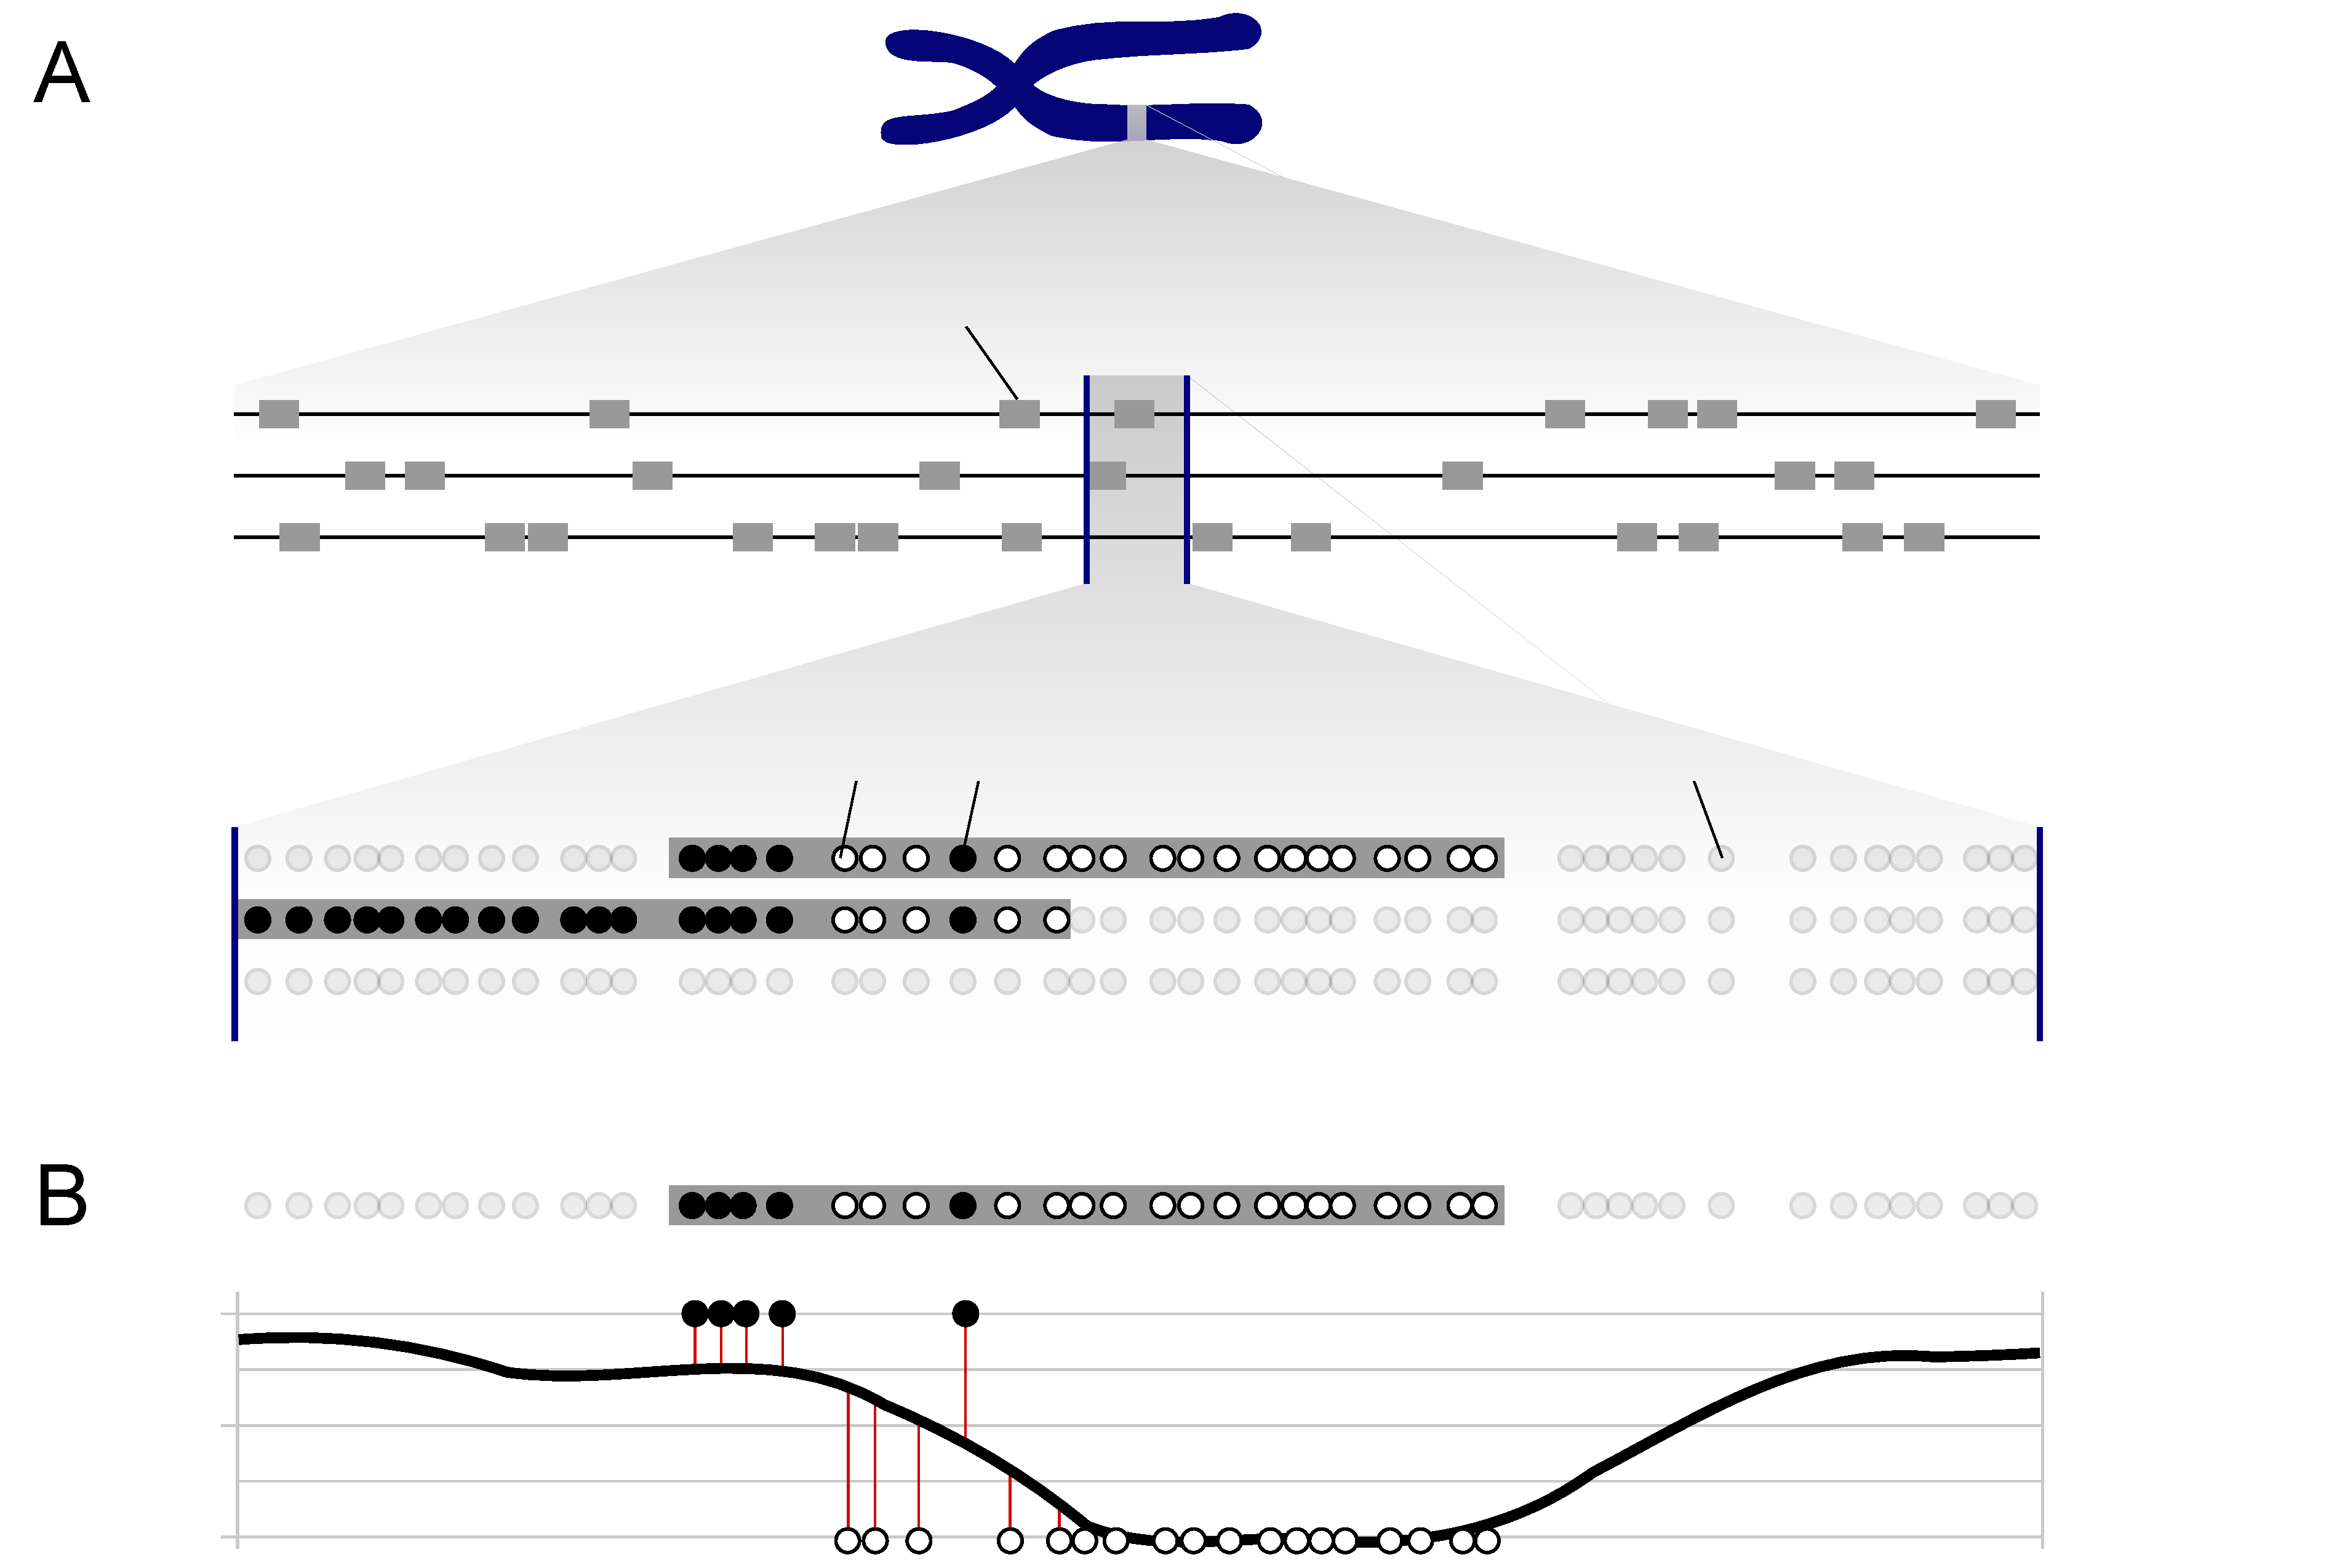
\includegraphics[width=0.7\textwidth]{figures/Fig_residuals_AB.pdf}\\
	\end{center}
	\caption{\small \textbf{Improved quantification of DNA methylation in a given genomic interval.}\\
		\textbf{(A)} Depicted is a genomic interval (between vertical blue lines) along a chromosome, for which DNA methylation is to be quantified.
		Two cells cover differing parts of the interval with one read each.
		If one simply counts for each cell which fraction of the covered CpG sites are methylated, one obtains very different values for the two cells.
		\textbf{(B)} By averaging each CpG site's methylation over all cells and subsequent smoothing, the thick black ``average methylation curve'' is obtained.
		To quantify the methylation of cell 1 from (A) relative to this average over all cells, we propose to use the cell's residuals to the smoothed curve (lengths of the vertical red lines) and take their average, counting residuals of methylated CpGs positive and residuals of unmethylated CpGs negative.}
	\label{fig:smoothres}
\end{figure*}


\begin{figure}[p]
	\begin{center}
		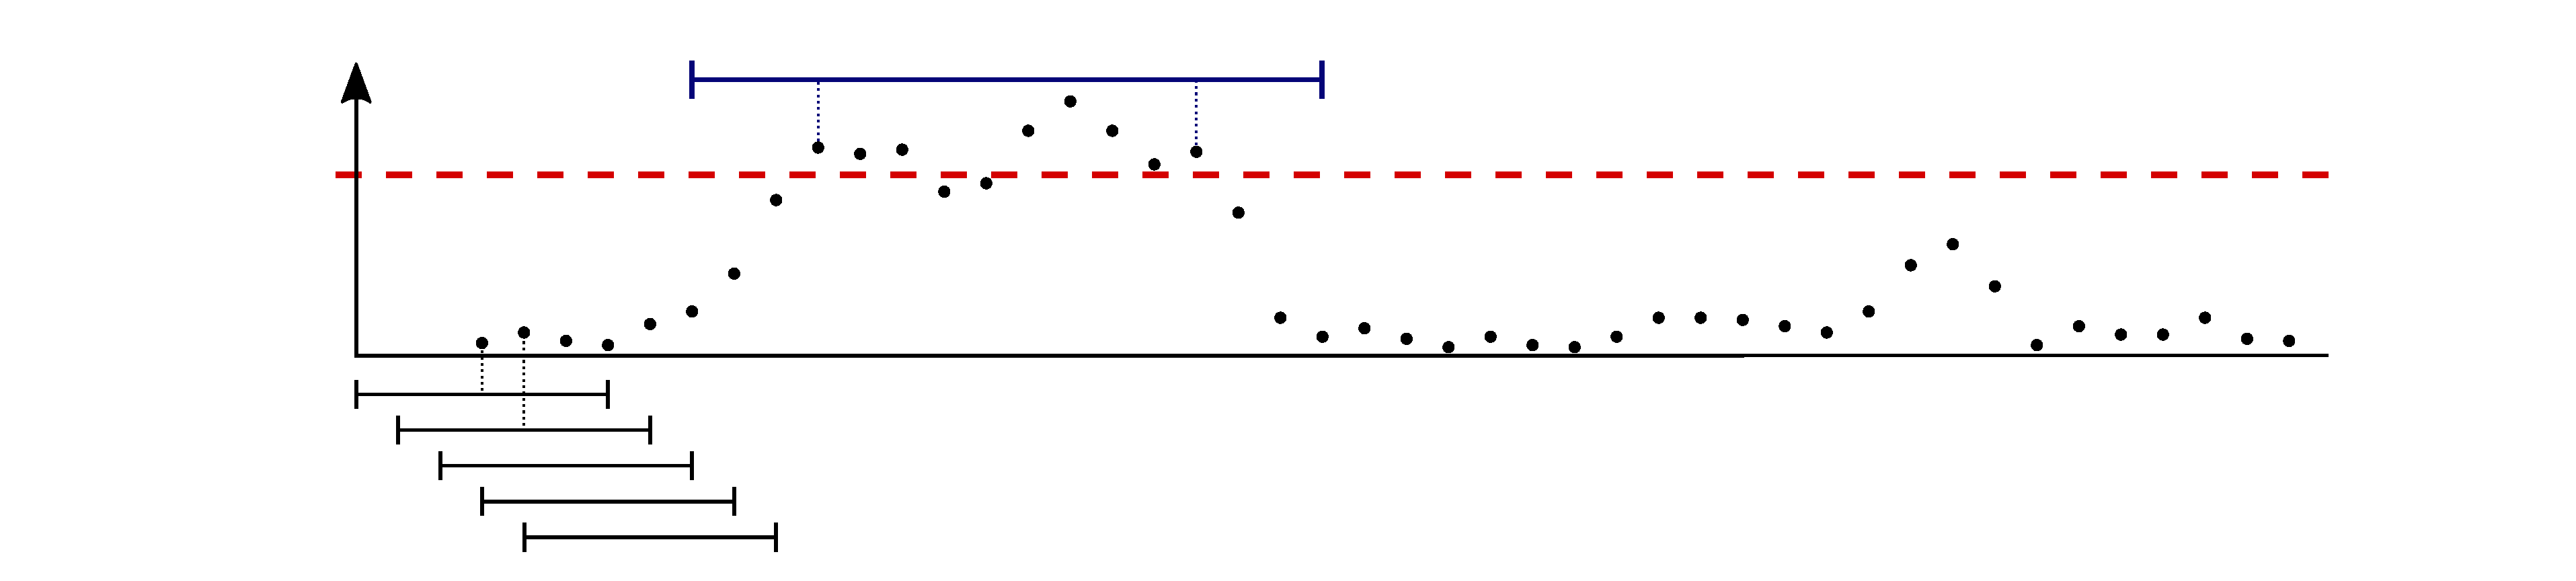
\includegraphics[width=.7\columnwidth]{figures/Fig_sliding.pdf}
	\end{center}
	\caption{\small \textbf{Finding variably methylated regions.}\\
		The chromosomes are divided up into overlapping windows (first five shown at the bottom), and for each window, the cells' methylation values are calculated as described and as depicted in Fig.~\ref{fig:smoothres}B.
		Then, the variance of these values is calculated (each point represents one of the overlapping windows), a threshold (dashed line) is chosen such that a chosen quantile of windows have a variance exceeding the threshold.
		Windows with above-threshold variance are merged if they overlap, yielding the ``variably methylated regions'' (VMRs).}
	\label{fig:vmr}
\end{figure}


\begin{figure*}[p]
	\begin{center}
		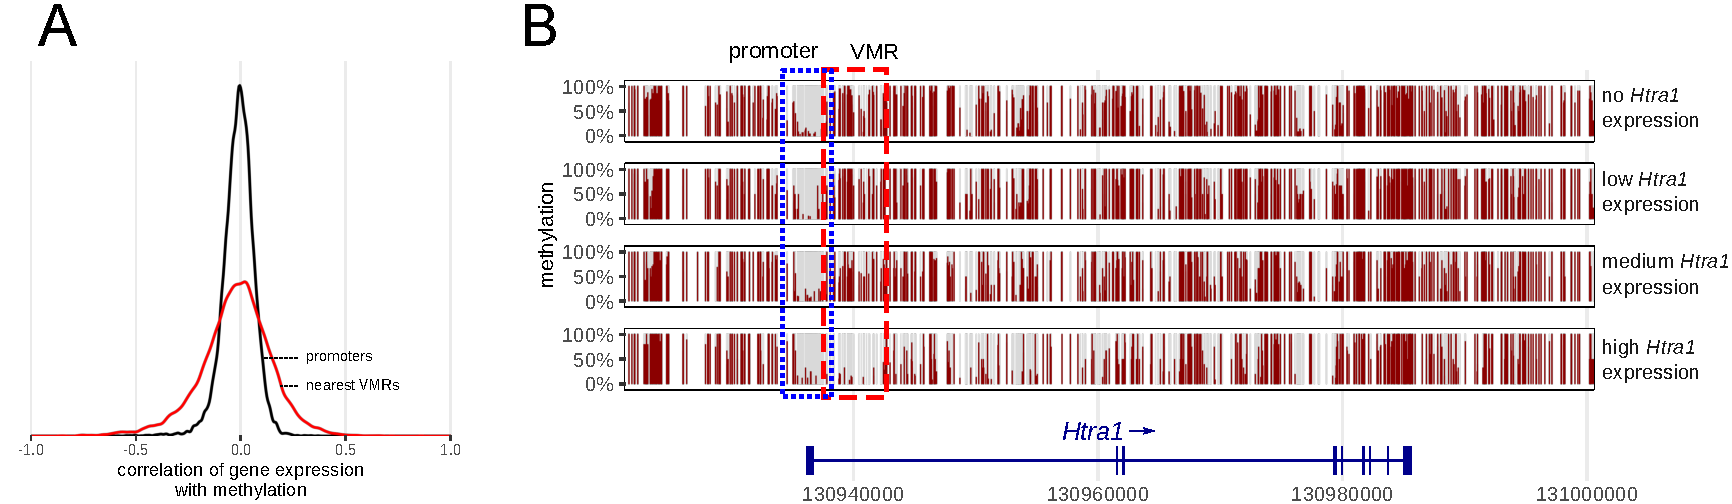
\includegraphics[width=\textwidth]{figures/Fig_correlation.pdf}
	\end{center}
	\caption{\small \textbf{Correlation of DNA methylation and gene expression}.\\
		\textbf{(A)} Distribution of Pearson correlations between gene expression and promoter methylation (black) and gene expression and methylation of the nearest VMR (red): for most promoters, correlation is weak.
		Promoters are defined as intervals \textpm2~kb around the TSS.
		\textbf{(B)} Mean methylation near the gene \textit{Htra1}.
		Cells are assigned to 4 groups based on \textit{Htra1} expression (group 0: cells with no \textit{Htra1} expression, groups 1-3: cells that express \textit{Htra1}, divided into three equally large groups with group 3 having the highest expression).
		Data from \citet{kremer_scnmt}.}
	\label{fig:correlation}
\end{figure*}

\begin{figure*}[p]
	\begin{center}
		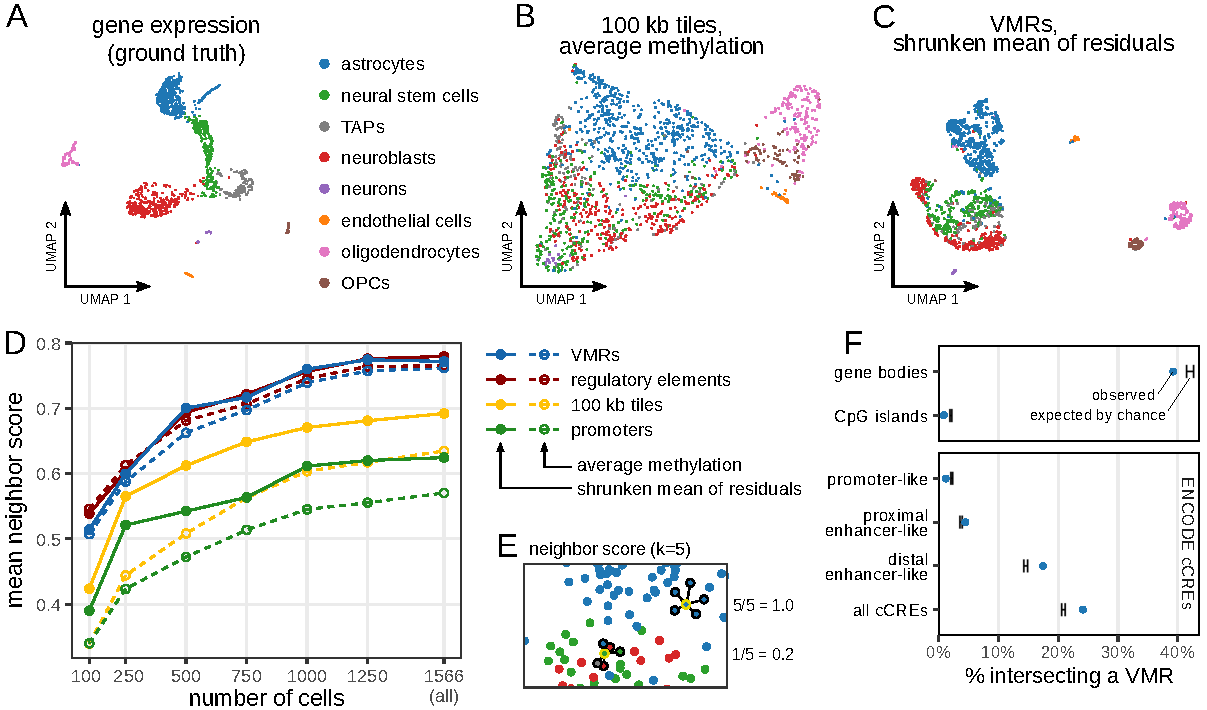
\includegraphics[width=0.9\textwidth]{figures/Fig_benchmark.pdf}
	\end{center}
	\caption{\small \textbf{Benchmark of our methods on single-cell multi-omic data of cells of the murine forebrain}.\\
		\textbf{(A)} Cell labels based on clustering of single-cell transcriptomes from \citet{kremer_scnmt}.
		\textbf{(B, C)} Exemplary UMAPs obtained when analyzing the data set with conventional methods based on genome tiling (B) or our proposed methods (C).
		\textbf{(D, E)} Mean degree of cell type separation (neighbor score, E, computed in 15-dimensional PC space) obtained when analyzing single-cell methylomes with different combinations of methods.
		Either VMRs, ENCODE regulatory elements, 100~kb genomic tiles or promoter regions (TSS\textpm2kb) were subjected to iterative PCA and UMAP.
		CpG methylation in these intervals was either quantified by averaging (dotted lines) or using the shrunken mean of the residuals as proposed in this work (solid lines).
		The full 1566-cell data set was sub-sampled to simulate smaller data sets (x axis).
		A higher neighbor score implies better separation of cell types inferred from single-cell transcriptomes of the same cells (A).
		\textbf{(F)} Proportion of VMRs (blue dots) that have at least 1~bp overlap with other genomic features.
		The black range illustrates the minimum and maximum overlap observed for 100 reshufflings of the VMRs to randomly chosen positions.
	}
	\label{fig:score}
\end{figure*}


\begin{figure*}[p]
	\begin{center}
		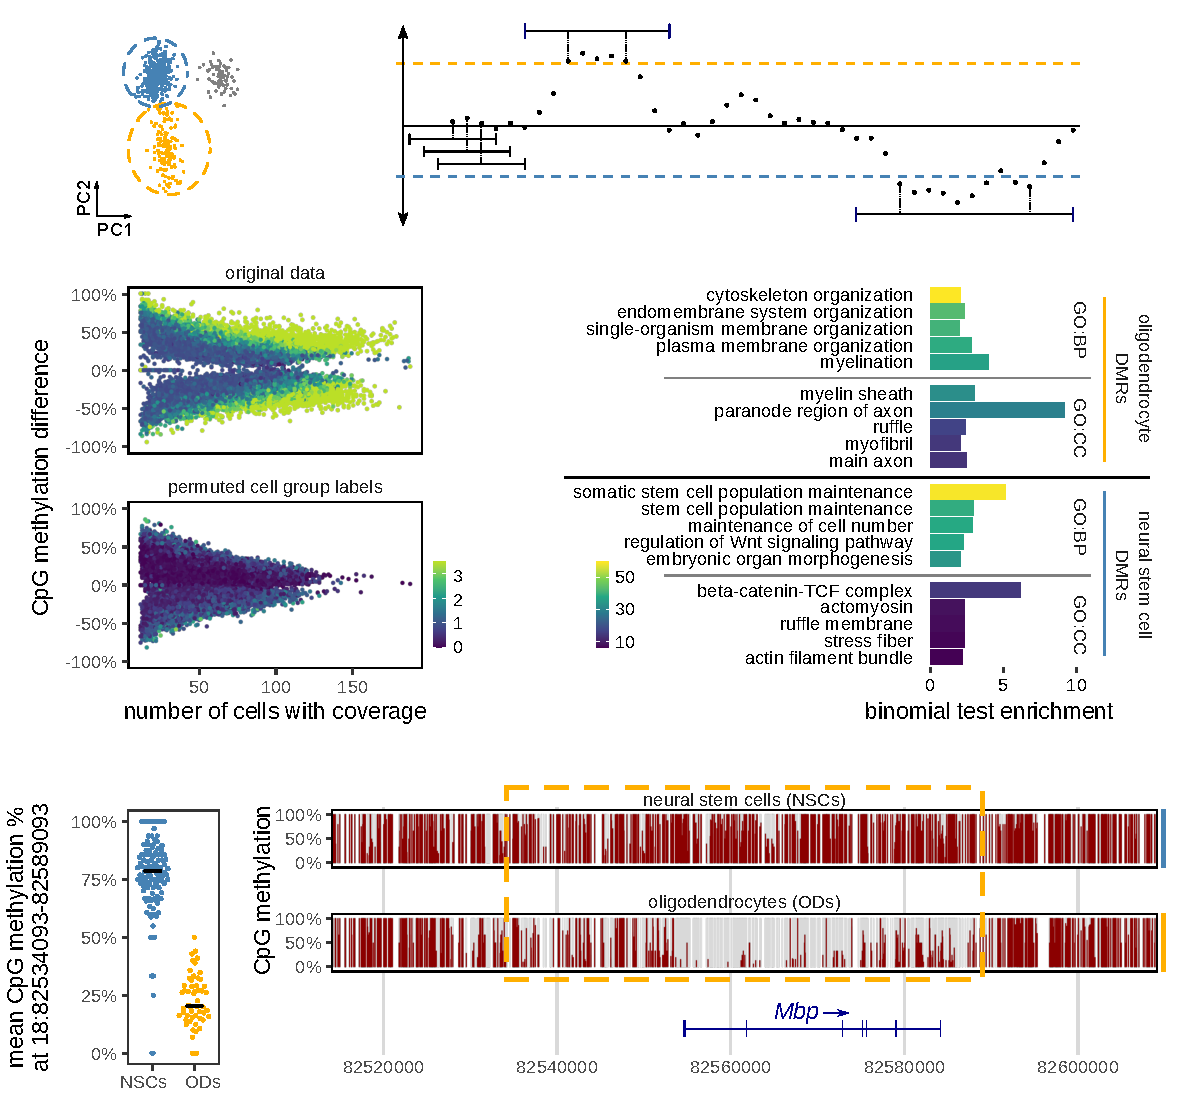
\includegraphics[width=.8\textwidth]{figures/Fig_DMRs.pdf}
	\end{center}
	\caption{\small \textbf{Detection of differentially methylated regions (DMRs).}\\
		\textbf{(A)} To identify DMRs, the chromosome is first divided into windows overlapping by a small and fixed size.
		For each window, the cell’s methylation values are calculated as described and as depicted in Fig.~\ref{fig:smoothres}B.
		Then the t statistic of these values is obtained as a measure of methylation difference between two groups of cells that were selected by the user (each point represents one of the windows).
		Upper and lower thresholds (dashed lines) are chosen such that a defined quantile of windows have a t statistic above or below the threshold.
		Windows exceeding either threshold are merged if they overlap, yielding DMRs that are lowly methylated in either group of cells.
		\textbf{(B)} DMRs detected between 58 oligodendrocytes (ODs) and 130 neural stem cells (NSCs) from \citet{kremer_scnmt} (top) and DMRs detected in the same data with randomly permuted cell labels (bottom, used to estimate FDR and determine adjusted p-values).
		\textbf{(C)} Enrichment of GO terms associated with DMRs lowly methylated in ODs (top) or NSCs (bottom).
		Depicted are the top 5 GO terms of the "Biological Process" (GO:BP) and "Cellular Component" (GO:CC) GO category, and their binomial test p-value (two-sided, not adjusted for multiple comparisons) and enrichment, as reported by GREAT \citep{mclean2010great}.
		\textbf{(D)} Mean methylation of NSCs and ODs at an exemplary DMR.
		Each point corresponds to a cell, black lines denote the median.
		\textbf{(E)} Detailed view of the DMR (yellow dashed rectangle) from C in pseudo-bulk samples consisting of NSCs or ODs.
		Vertical bars represent CpG sites.
	}
	\label{fig:dmr}
\end{figure*}



\begin{figure*}[p]
	\begin{center}
		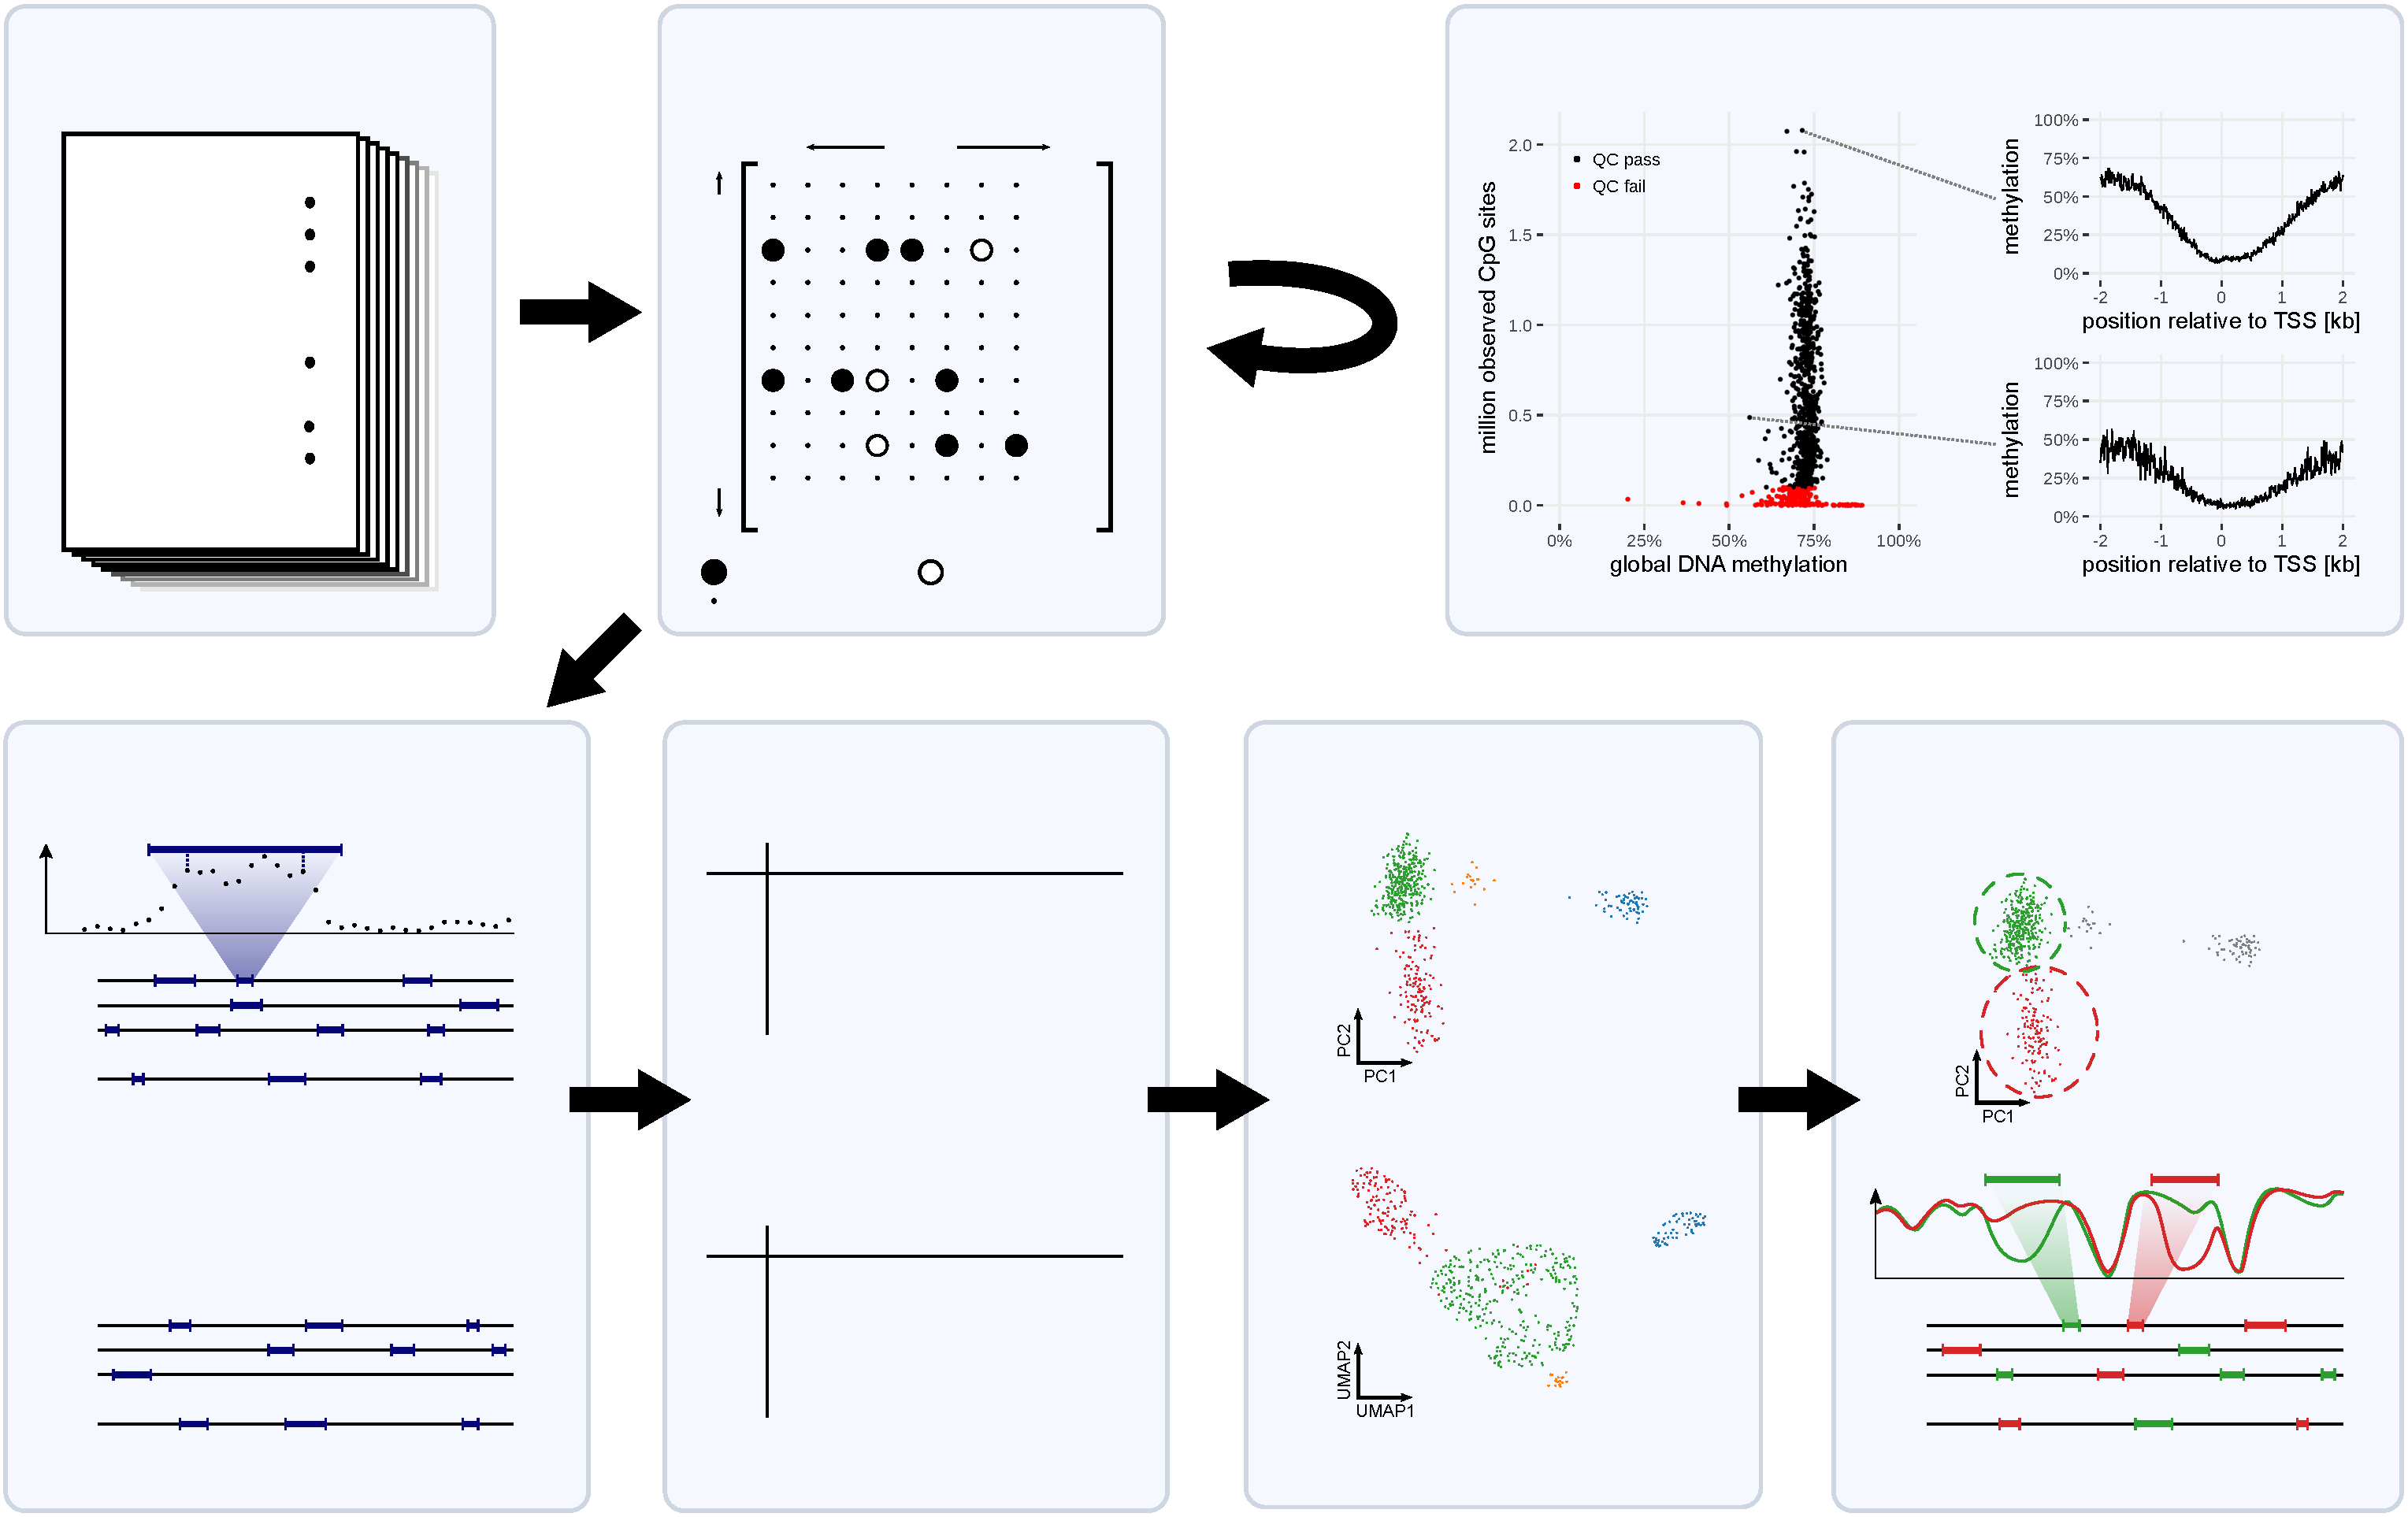
\includegraphics[width=.8\textwidth]{figures/Fig_workflow.pdf}
	\end{center}
	\caption{\small \textbf{Overview of the functionalities implemented in the \textit{MethSCAn} package.}\\
		Common bisulfite sequencing mappers produce one methylation report file per cell.
		As it is inconvenient to work with thousands of text files, \texttt{methscan prepare} first stores their contents in a compressed format optimized for efficient access to genomic intervals.
		This command also produces cell-wise summary statistics that can be used to discard low-quality cells with \texttt{methscan filter}.
		The quality of each cell can furthermore be assessed by visualizing the average methylation around transcription start sites, which are known to show a characteristic dip in mammalian genomes, using \texttt{methscan profile}.
		This command can also visualize methylation at other genomic features of interest, such as enhancers or transcription factor binding sites.
		To obtain a methylation matrix analogous to scRNA-seq count matrices, the user must first decide in which genomic intervals methylation should be quantified.
		The user may either provide genomic regions of \emph{a priori} interest as a BED file, or they may choose to discover VMRs (variably methylated regions) in the data with \texttt{methscan scan}.
		The \texttt{methscan matrix} command then quantifies methylation at these genomic intervals in all cells.
		It provides two metrics:
		the simple percentage of methylated CpG sites and our proposed measure, the shrunken mean of the residuals, which is more robust to variation in sequencing coverage and stochastic differences in read position between cells.
		The resulting methylation matrix can then serve as input for established methods used for the exploration of single-cell data, such as dimensionality reduction and cell clustering.
		Finally, after annotation and exploration of the data set, the user may specify two groups of cells for DMR (differentially methylated region) detection with \texttt{methscan diff}.
		This command produces a BED file listing the genome coordinates, adjusted p-values, as well as several other metrics associated with DMRs.
		These DMRs may then be associated with nearby genes, or used for GO enrichment with tools such as GREAT \citep{mclean2010great} to enable functional interpretation.
	}
	\label{fig:workflow}
\end{figure*}



\clearpage
\section*{Methods}

\subsection*{Raw data}

Let us write $x_{ij}$ for the methylation status of CpG $i$ in cell $j$.
The index $i$ runs over all CpG positions present in the genome, the index $j$ over all cells in the assay.
We write $x_{ij}=0$ if position $i$ was found to be unmethylated in cell $j$ by bisulfite sequencing, $x_{ij}=1$ if it was methylated, and $x_{ij}=\text{NA}$ if position $i$ was not covered by reads from cell $j$ and the methylation status is therefore not available (``NA'').

These values can be readily obtained from single-cell bisulfite sequencing data using tools like Bismark.

If multiple reads from the same cell cover a position, these will typically be PCR duplicates of each other and hence agree.
Of course, the two alleles of a CpG may rarely differ in their methylation status.
While it is in principle possible that one obtains discordant reads stemming from the same position on both the paternal and the maternal chromosomes of the same cell, this is so unlikely that we can ignore the case.
Hence, whenever the methylation caller reports multiple reads covering the same position in the same cell, we set $x_{ij}$ to 0 or 1 whenever all reads agree.
When there is disagreement, we put $x_{ij}=\text{NA}$ by default, or optionally follow the majority of reads whenever possible.

For later use: We define $C$ as the set of all cells in the assay (i.e., $C$ is the index set for the cell indices $j$).
Moreover, we define $C_i\subset C$ as the set of all those cells $j$ that have reads covering position $i$,
\[ C_i=\{j\in C: x_{ij}\neq\text{NA}\}.\]
Conversely, we define $G_j$ as the set of all the CpG positions $i$ covered by reads from cell $j$ 
\[ G_j=\{i: x_{ij}\neq\text{NA}\}.\]

\subsection*{Data storage}

The function \texttt{methscan prepare} reads a set of methylation files (e.g. produced by Bismark) and produces one file per chromosome.
These files store the matrix $x$, where each column represents a cell and each row represents a base pair, in a space-efficient format as follows:
$x$ is represented as a SciPy sparse matrix \citep{SciPy}, encoding the actual values 0, 1, and NA as -1, 1, and 0, respectively.
Since the vast majority of values in this matrix are missing due to the sparsity of scBS data (and because rows for base-pairs not corresponding to a CpG site contain no data), we encode missing values as zero and then store the data in Compressed Sparse Row (CSR) format.
This format does not explicitly store zeroes (here: missing values) and is optimized for row-wise access, which results in significant compression and allows fast access to the methylation status of genomic intervals.
In all that follows here, any mention of $x$ will, however, always mean the encoding as $x_{ij}\in\{0,1,\text{NA}\}$.

\subsection*{Smoothing}

For each CpG position $i$, we write 
\[\overline{x}_i=\langle x_{ij} \rangle_{j\in C_i} = \frac{1}{|C_i|}\sum_{j\in C_i} x_{ij}\] 
for the average methylation at position $i$, where $\langle\cdot\rangle$ denotes averaging, and the average runs over all the cells $j\in C_i$, i.e.
over those cells for which methylation data is available for position $i$.

We then run a kernel smoother over these per-position averages to obtain the smoothed averages $\tilde x_i$.
Specifically, we use
\[ \tilde x_i = \frac{\sum_{i'} \overline x_{i'}\, k_h(d_{ii'})}{\sum_{i'} k_h(d_{ii'})},\]
i.e., $\tilde x_i$ is the weighted average over the per-position averages $\overline{x}_{i'}$, taken over the CpG sites $i'$ in the neighborhood of $i$, and weighted using a smoothing kernel $k_h$ with bandwidth $h$.
Here, $d_{ii'}$ is the distance between CpG positions $i$ and $i'$, measured in base pairs, $h$ is the smoothing bandwidth in base pairs (by default, $h=1000$), and $k_h$ is the tricube kernel,

\[ k_h(d) = \left\{
\begin{aligned}
    &\left(1-|d/h|^3\right)^3 &\text{for } |d|<h \\
    &\,0 &\text{otherwise}.
\end{aligned}
\right.
\]

\subsection*{Methylation for an interval}

Next, we discuss averaging methylation over a range of CpG sites.

Given an interval $I$ on the chromosome, we wish to quantify the average methylation $m_{Ij}$ of the CpG sites within the interval for cell $j$.
If we interpret $I$ as the set of CpG positions $i$ in the interval, we may write

\[ m_{Ij} = \left< x_{ij} \right>_{i\in I\cap G_j}.\]

Here, the average runs over all those sites $i$ that lie within the interval $I$ and are covered by reads from cell $j$.

If we wish to compare cells, it can be helpful to center this quantity by subtracting its average:

\[ z_{Ij} = m_{Ij} - \langle m_{Ij'}\rangle_{j'\in C}.\]

As an alternative, we suggest to consider the residuals of the individual CpG methylation values $x_{ij}$ from the smoothed average $\tilde x_i$,
\[ r_{ij} = x_{ij} - \tilde x_i, \]
and averaging over these, obtaining
\begin{equation} 
r_{Ij} = \frac{1}{|I\cap C_i|+1}\sum_{i\in I\cap C_i}\left( x_{ij} - \tilde x_i \right).
\label{avgres}
\end{equation}

This is a shrunken average, with denominator $n+1$.
This extra pseudocount has the effect of shrinking the value towards the ``neutral'' value 0, with the shrinkage becoming stronger if the data is ``weak'' because the number $|I\cap C_i|$ of positions covered by reads from cell $j$  is low.
In the extreme case of none of the reads from cell $j$ covering $I$, the sum becomes 0 and the denominator 1, i.e.
$r_{Ij}=0$ in this case.

\subsection*{Finding variably methylated regions}

For any interval $I$, we denote by $v_I$ the variance of its residual averages $r_{Ij}$:

\begin{equation} 
v_I = \frac{1}{|C_I|}\sum_{j\in C_I}\left( r_{Ij} - \langle r_{Ij'}\rangle_{j'\in C_I} \right)^2, \label{var}
\end{equation}

where the average runs only over the set $C_I=\bigcup_{i\in I}C_i$ of those cells $j$ which have reads covering interval I.

To find VMRs, we define intervals $I_1, I_2, ...$, all of the same width, and with step-wise increasing starts, then calculate $v_1, v_2, ...$ for these intervals.
We then mark the intervals with the 2\% highest variances.
We take the union of all these intervals, split the union into connected components, and call each component a VMR.
Putting that last step in other words:
We take all the intervals with variance in the top 2-percentile, fuse intervals that overlap and call the regions thus obtained the VMRs.

\subsection*{Finding differentially methylated regions}

When searching for DMRs, we compare two groups of cells, whose index sets we denote with $C_\text{A}$ and $C_\text{B}$.
For a given interval $I$, we calculate the mean each of the mean shrunken residuals $r_{ij}$ (see Eq.~(\ref{avgres})) over the cells $j$ in each of the two groups,
\[ \mu^g_I = \langle r_{Ij} \rangle_{j\in g},\qquad g=\text{A},\text{B}. \]

We also calculate a variance as in Eq.(\ref{var}):
\[ v^g_I = \frac{1}{|C_\text{g}|-1}  \sum_{j\in g} \left( r_{Ij} - \mu_I^g \right)^2, 
\qquad g=\text{A},\text{B}.\]

From this, we calculate Welch's t statistic as usual:
\[ t_I = \frac{\mu^\text{A}_I - \mu^\text{B}_I}{\sqrt{\frac{v^\text{A}_I}{|C_A|} + \frac{v^\text{B}_I}{|C_B|}}}.\]

In order to find candidate DMRs, we again define overlapping and stepwise shifted intervals $I_1, I_2, \dots$ as for the VMRs and calulate t statistics $t_1, t_2, \dots$ for these.
As before, we take the top 2-percentile of these values, fuse intervals that overlap and call the regions thus obtained candidate DMRs.
We repeat the procedure for the bottom 2-percentile to get the candidate DMRs for the other sign.

Next, we need to check these candidate DMRs for statistical significance.
We first remind the readers here that, as this is a within-sample analysis, and cells, not samples, are the statistical unit.
Therefore, a call as significant implies that the same DMR is likely to be called again if we repeated the analysis with another set of cells taken from the same biological sample, not that it would generalize to further samples.
This fact, although often overlooked, is common to all within-sample analyses in the single-cell fields, e.g. also to the differential expression tests performed in scRNA-seq analyses to find marker genes that differentiate clusters.

It may seem that we could use the standard procedure for the Welch t-test here, i.e.\ use the Welch-Satterthwaite formula to get an approximate degree of freedom and then calculate the tail probability of the corresponding t distribution.
However, this is unlikely to hold for two reasons:
First, the Welch-Satterthwaite degrees of freedom are only based on the number of cells per group and do not account for the fact that the read coverage might vary from cell to cell.
Second, the fusing of the DMRs obtained in the scanning step to obtain fused candidate DMRs would invalidate subsequent p-value based adjustment for multiple testing.

Therefore, we have instead implemented a permutation procedure, which works as follows:
We randomly shuffle the assignment of the cells in $C_\text{A}\cup C_\text{A}$ to either of the two groups and then rerun the whole procedure, i.e., the scanning step, the DMR fusing and the calculation of t values from the (potentially fused) candidate DMRs.
This needs to be done for a sufficiently large number of permutations.
Running through the whole genome for each permutation would be too computationally expensive.
Instead, we go through the genome only once, but reshuffle the group labels every 2~Mbp.

All the t values obtained from this permutation procedure are taken together to get an empirical null distribution.
Then, we can use this null distribution to control false discovery rate (FDR) by applying the Benjamini-Hochberg procedure in its p-value-free form:
Let us write $T$ for the set of all t values obtained from the ``real'' assignment of cells to group labels and $T_0$ from the set of all t values obtained from the shuffled assignments, i.e., the empirical null distribution.
To adjust a specific t value $t_i\in T$, we calculate
\[ p^\text{adj}_i = \frac{ \left|\left\{t_j\in T_0\mid|t_j| > |t_i| \right\}\right| \big/ |T_0|}
{ \left|\left\{t_j\in T\mid|t_j| > |t_i| \right\}\right| \big/ |T|}.\]

In words: we calculate which fraction of the null t values is greater than t by absolute value, and which fraction of the real t values is.
The ratio gives us the false discovery rate we should expect if we used the t value as threshold.


\subsection*{Calculating cell to cell distances}

Given a set, $\mathcal{V}=\{I^\text{v}_1,I^\text{v}_2,\dots\}$, of intervals corresponding to VMRs, we get a relative methylation fraction $r_{ij}$ for each VMR $I^\text{v}_i$ and each cell $j$ from Eq.\ (\ref{avgres}).
The matrix thus obtained can then be centered and used as input for a PCA.
If we calculate the top $R$ principal components, we thus obtain for each cell $j$ an $R$-dimensional principal component vector $\mathbf{x}^\text{P}_j$.
For any two cells $j$, $j'$, we use the Euclidean distance $\|\mathbf{x}^\text{P}_j - \mathbf{x}^\text{P}_{j'}\|$ as the measure of dissimilarity of the two cells.
Thus, the matrix of PC scores can be used as input to dimension reduction methods like t-SNE or UMAP, and to clustering methods like the Louvain or Leiden algorithm, which require such a matrix as input to the approximate nearest neighbor (ANN) finding algorithm that is their first step.

\subsection*{PCA with iterative imputation}

Whenever a region is not covered by any read in a cell, the corresponding data entry in the input data matrix for PCA will be missing.
The standard approach to calculate PCA, commonly done using the IRLBA algorithm \citep{Baglama2005}, is not suited to deal with missing data.
We circumvent this issue by simply using the PCA itself to impute the missing value in an approach that we call "iterative PCA").

Let us write $A$ for the matrix to which the PCA is to be applied, with the features (here: regions) represented by the matrix rows.
The matrix has already been centered, i.e., $\sum_i a_{ij}=0$.
To establish notation, we remind the reader that performing a PCA on A means finding the singular value decomposition (SVD), $A=UDR^\top$, with $D$ diagonal and $U$ and $R$ orthonormal.
The PCA scores are contained in $X=UD$, the loadings in $R$.
To reconstruct the input data $A$ from the PCA representation, one may use $A=XR^\top$, i.e., $a_{ij}=\sum_r x_{ir} r_{jr}$, where the equation is exact if $r$ runs over all principal components and approximate if it is truncated to the leading ones.

Our iterative imputation strategy is now simply the following: we first replace all missing values in the row-centered input matrix $A$ with zeroes and perform the (truncated) PCA.
Then, we use the PCA predictions for the missing values, i.e., the $a_{ij}=\sum_r x_{ir} r_{jr}$, as refined stand-ins for the missing values in $A$ and run PCA once more.
This can now be iterated until convergence.

We note that similar approaches have also been used elsewhere \citep{josse2012}.


\subsection*{Analysis of scBS datasets for benchmarks}
To analyze scBS data from \citet{kremer_scnmt}, single-cell CpG methylation reports from all conditions were first stored with \texttt{methscan prepare} and then smoothed with \texttt{methscan smooth} using the default bandwidth of 1000~bp.
This data was then analysed multiple times with different combinations of analysis methods, namely four ways to divide the genome into intervals, two ways to quantify methylation in these intervals, and four approaches for dimensionality reductions.
The following four sets of genomic intervals were used:
VMRs, obtained with \texttt{methscan scan} using the current default options (bandwidth $=2000$, stepsize $=10$, variance threshold $= 0.02$, minimum cell requirement $=6$);
adjacent tiles of 100~kb width;
promoter regions as defined by the \textpm2~kb domain around the TSS of coding genes;
and candidate cis-regulatory regions annotated by the ENCODE consortium \citep{encode2020expanded}.
Methylation was quantified either by averaging binary methylation values, or by calculating the shrunken mean of the residuals as described earlier.

We used four different approaches for dimensionality reduction. Three of them involve imputation of missing values followed by PCA:
The first approach, iterative PCA, was described earlier.
Second, "PCA on high-quality features" imputes missing values with the mean methylation level of a the given interval, while only retaining high-quality features selected as in \citet{luo2017single}:
We selected tiles spanning $\ge20$ CpG sites and with sequencing coverage in at least 70\% of cells.
We then imputed missing values with the mean of each tile, centered the values, and performed PCA.
The third approach, "mean-imputed PCA" is identical to approach two, but without the quality-filtering step.
Lastly, we used MOFA+ with default parameters instead of PCA, which does not require imputation of missing values. 
In all four cases we reduced the dimensionality of the input data to 15 PCs or MOFA factors. In some cases MOFA+ returned a smaller number of factors, since some of the requested 15 had zero variance.
For visualization, these 15 PCs or factors were subjected to UMAP with parameters min\_dist $=0.2$, init $=$ ``spca''.
To flexibly adapt to data sets of different sizes, we set n\_neighbors  $=\frac{\sqrt{n}}{1.5}$ (rounded to the nearest integer), where $n$ is the total cell number.

The same analysis was repeated for three additional scBS data sets \citep{luo2017single, bian2018single, argelaguet2019gastru}, and for smaller data sets generated by randomly sub-sampling cells separately from these data sets.

VMRs that intersect protein-coding gene bodies, CpG islands (from the UCSC genome browser) or cCREs were quantified by subtracting VMRs with at least one bp of overlap using \texttt{bedtools} \texttt{subtract} \texttt{-A} \citep{quinlan2010bedtools} and counting the remaining VMRs.


To test our DMR detection approach, we selected oligodendrocytes and NSCs from healthy wild type mice of \citet{kremer_scnmt} and ran \texttt{methscan diff} with default parameters.
For GO enrichment analysis, DMRs with adjusted $p<0.01$ were uploaded to GREAT 4.0.4 \citep{mclean2010great} with the association rule "basal plus extension, 0~bp upstream, 20~kb downstream, 1~Mbp max extension, curated regulatory domains included".

\subsection*{Mean neighbor score} \label{methods:score}
To assess performance of our methods, we employed a score that quantifies how well cell types (or cell states) are separated in 15-dimensional PCA space.
For data from \citet{luo2017single}, we used cell type labels that the authors manually curated based on CH-methylation.
For the multi-omic data set, we repeated the single-cell transcriptomics analysis described in \citet{kremer_scnmt} with two adjustments:
We did not filter off-target cells such as endothelial cells, and we annotated cell types using Leiden clustering with the Seurat \citep{seurat5} function \texttt{FindClusters(resolution = 0.1)}.
The score, based on the $\Gamma$-score \citep{Kireeva_2014}, varies between 0 and 1, where higher scores reflect better separation of cell types.
For each cell $j$, we count how many of its $k$ nearest neighbors have been assigned to the same cell type as cell $j$.
We denote this count $a^k_j$, where we have chosen $k=\frac{\sqrt{n}}{1.5}$, rounded.
The overall score used to evaluate a given combination of methods is then simply the mean of all cell-wise scores.

\subsection*{Correlation of DNA methylation and gene expression}
To assess correlation between gene expression and the methylation status of VMRs or promoters, we first detected VMRs with \texttt{methscan scan --bandwidth 1000 --var-threshold 0.05}.
We then quantified DNA methylation at VMRs and promoters with \texttt{methscan matrix}.
We defined promoters as $\pm2000$~bp regions centered on a genes transcription start site (TSS).
When multiple TSSs were annotated, we chose the TSS of the "principal" isoform \citep{appris}.
Log-normalized expression values reported by \citet{kremer_scnmt} were then correlated with methylation of the gene's promoter, or with methylation of the VMR closest to the gene body.
When multiple VMRs intersected the gene body, we chose the VMR with the highest methylation variance.
As a measure of methylation we used the shrunken mean of the residuals.
We omitted lowly expressed genes (with scRNA-seq counts in $<5\%$ of cells) and promoters and VMRs with low scBS coverage (in $<10$ cells).

MethSCAn was implemented in Python 3.8 using the packages NumPy 1.20.1, SciPy 1.6.1, numba 0.53.0 and Pandas 1.2.3. Benchmarks were performed on MethSCAn version 0.6.2 using Snakemake 7.26 and analyzed/visualized with tidyverse 1.3.1 packages. 
\vspace{1.4ex}
\noindent\hfil\rule{.6\columnwidth}{.2pt}\hfil



\subsection*{Data Availability}

All data used to benchmark and showcase the \textit{MethSCAn} software is publicly available under the following NCBI Gene Expression Omnibus accessions:
Single-cell multi-omics of the murine forebrain \citep{kremer_scnmt}: \texttt{GSE210806};
mouse neurons \citep{luo2017single}: \texttt{GSE97179};
colorectal cancer \citep{bian2018single}: \texttt{GSE97693};
mouse gastrulation \citep{argelaguet2019gastru}: \texttt{GSE121708};
100k brain cells \citep{liu2021dna}: \texttt{GSE132489}.


\subsection*{Code Availability}

\textit{MethSCAn} is free and open source.
The package is available on the Python Package Index (PyPI) and can be installed with the Python package installer \texttt{pip}.
The source code is hosted at \href{https://github.com/anders-biostat/MethSCAn}{https://github.com/anders-biostat/MethSCAn}, where we also provide detailed documentation including a tutorial that demonstrates a complete \textit{MethSCAn} analysis on an example data set.


\begin{thebibliography}{31}
	\providecommand{\natexlab}[1]{#1}
	\providecommand{\url}[1]{\texttt{#1}}
	\expandafter\ifx\csname urlstyle\endcsname\relax
	\providecommand{\doi}[1]{doi: #1}\else
	\providecommand{\doi}{doi: \begingroup \urlstyle{rm}\Url}\fi
	
	\bibitem[Frommer et~al.(1992)Frommer, McDonald, Millar, Collis, Watt, Grigg,
	Molloy, and Paul]{Frommer_1992}
	M.~Frommer, L.~E. McDonald, D.~S. Millar, C.~M. Collis, F.~Watt, G.~W. Grigg,
	P.~L. Molloy, and C.~L. Paul.
	\newblock A genomic sequencing protocol that yields a positive display of
	5-methylcytosine residues in individual {DNA} strands.
	\newblock \emph{Proceedings of the National Academy of Sciences}, 89\penalty0
	(5):\penalty0 1827--1831, mar 1992.
	\newblock \doi{10.1073/pnas.89.5.1827}.
	\newblock URL \url{https://doi.org/10.1073/pnas.89.5.1827}.
	
	\bibitem[Smallwood et~al.(2014)Smallwood, Lee, Angermueller, Krueger, Saadeh,
	Peat, Andrews, Stegle, Reik, and Kelsey]{Smallwood_2014}
	S{\'{e}}bastien~A Smallwood, Heather~J Lee, Christof Angermueller, Felix
	Krueger, Heba Saadeh, Julian Peat, Simon~R Andrews, Oliver Stegle, Wolf Reik,
	and Gavin Kelsey.
	\newblock Single-cell genome-wide bisulfite sequencing for assessing epigenetic
	heterogeneity.
	\newblock \emph{Nature Methods}, 11\penalty0 (8):\penalty0 817--820, jul 2014.
	\newblock \doi{10.1038/nmeth.3035}.
	\newblock URL \url{https://doi.org/10.1038/nmeth.3035}.
	
	\bibitem[Hu et~al.(2016)Hu, Huang, An, Du, Hu, Xue, Zhu, Wang, Xue, and
	Fan]{scMTseq}
	Youjin Hu, Kevin Huang, Qin An, Guizhen Du, Ganlu Hu, Jinfeng Xue, Xianmin Zhu,
	Cun-Yu Wang, Zhigang Xue, and Guoping Fan.
	\newblock Simultaneous profiling of transcriptome and {DNA} methylome from a
	single cell.
	\newblock \emph{Genome Biology}, 17\penalty0 (1):\penalty0 1--11, 2016.
	\newblock \doi{10.1007/978-1-4939-9240-9_21}.
	
	\bibitem[Clark et~al.(2018)Clark, Argelaguet, Kapourani, Stubbs, Lee,
	Alda-Catalinas, Krueger, Sanguinetti, Kelsey, Marioni, Stegle, and
	Reik]{Clark2018}
	Stephen~J. Clark, Ricard Argelaguet, Chantriolnt-Andreas Kapourani, Thomas~M.
	Stubbs, Heather~J. Lee, Celia Alda-Catalinas, Felix Krueger, Guido
	Sanguinetti, Gavin Kelsey, John~C. Marioni, Oliver Stegle, and Wolf Reik.
	\newblock {scNMT}-seq enables joint profiling of chromatin accessibility {DNA}
	methylation and transcription in single cells.
	\newblock \emph{Nature Communications}, 9\penalty0 (1), February 2018.
	\newblock \doi{10.1038/s41467-018-03149-4}.
	\newblock URL \url{https://doi.org/10.1038/s41467-018-03149-4}.
	
	\bibitem[Hao et~al.(2023)Hao, Stuart, Kowalski, Choudhary, Hoffman, Hartman,
	Srivastava, Molla, Madad, Fernandez-Granda, and Satija]{seurat5}
	Yuhan Hao, Tim Stuart, Madeline~H Kowalski, Saket Choudhary, Paul Hoffman,
	Austin Hartman, Avi Srivastava, Gesmira Molla, Shaista Madad, Carlos
	Fernandez-Granda, and Rahul Satija.
	\newblock Dictionary learning for integrative, multimodal and scalable
	single-cell analysis.
	\newblock \emph{Nature Biotechnology}, 2023.
	\newblock \doi{10.1038/s41587-023-01767-y}.
	
	\bibitem[Wolf et~al.(2018)Wolf, Angerer, and Theis]{Wolf_2018}
	F.~Alexander Wolf, Philipp Angerer, and Fabian~J. Theis.
	\newblock {SCANPY}: large-scale single-cell gene expression data analysis.
	\newblock \emph{Genome Biology}, 19:\penalty0 15, 2018.
	\newblock \doi{10.1186/s13059-017-1382-0}.
	
	\bibitem[Luo et~al.(2017)Luo, Keown, Kurihara, Zhou, He, Li, Castanon, Lucero,
	Nery, Sandoval, et~al.]{luo2017single}
	Chongyuan Luo, Christopher~L Keown, Laurie Kurihara, Jingtian Zhou, Yupeng He,
	Junhao Li, Rosa Castanon, Jacinta Lucero, Joseph~R Nery, Justin~P Sandoval,
	et~al.
	\newblock Single-cell methylomes identify neuronal subtypes and regulatory
	elements in mammalian cortex.
	\newblock \emph{Science}, 357\penalty0 (6351):\penalty0 600--604, 2017.
	\newblock \doi{10.1126/science.aan3351}.
	
	\bibitem[Bird(1986)]{bird1986cpg}
	Adrian~P Bird.
	\newblock {CpG-rich} islands and the function of {DNA} methylation.
	\newblock \emph{Nature}, 321\penalty0 (6067):\penalty0 209--213, 1986.
	\newblock \doi{10.1038/321209a0}.
	
	\bibitem[Argelaguet et~al.(2019)Argelaguet, Clark, Mohammed, Stapel, Krueger,
	Kapourani, Imaz-Rosshandler, Lohoff, Xiang, Hanna,
	et~al.]{argelaguet2019gastru}
	Ricard Argelaguet, Stephen~J Clark, Hisham Mohammed, L~Carine Stapel, Christel
	Krueger, Chantriolnt-Andreas Kapourani, Ivan Imaz-Rosshandler, Tim Lohoff,
	Yunlong Xiang, Courtney~W Hanna, et~al.
	\newblock Multi-omics profiling of mouse gastrulation at single-cell
	resolution.
	\newblock \emph{Nature}, 576\penalty0 (7787):\penalty0 487--491, 2019.
	\newblock \doi{10.1038/s41586-019-1825-8}.
	
	\bibitem[Kremer et~al.(2022)Kremer, Cerrizuela, Al~Shukairi, Ellinger, Straub,
	Dehler, Korkmaz, Weichenhan, Plass, Anders, and
	Martin-Villalba]{kremer_scnmt}
	Lukas P.~M. Kremer, Santiago Cerrizuela, Mohammad~E Al~Shukairi, Tobias
	Ellinger, Jannes Straub, Sascha Dehler, Aylin Korkmaz, Dieter Weichenhan,
	Christoph Plass, Simon Anders, and Ana Martin-Villalba.
	\newblock Single-cell triple-omics uncovers {DNA} methylation as key feature of
	stemness in the healthy and ischemic adult brain.
	\newblock \emph{bioRxiv preprint}, 2022.
	\newblock \doi{10.1101/2022.07.13.499860}.
	
	\bibitem[Moore et~al.(2020)Moore, Purcaro, Pratt, Epstein, Shoresh, Adrian,
	Kawli, Davis, Dobin, et~al.]{encode2020expanded}
	Jill~E Moore, Michael~J Purcaro, Henry~E Pratt, Charles~B Epstein, Noam
	Shoresh, Jessika Adrian, Trupti Kawli, Carrie~A Davis, Alexander Dobin,
	et~al.
	\newblock Expanded encyclopaedias of {DNA} elements in the human and mouse
	genomes.
	\newblock \emph{Nature}, 583\penalty0 (7818):\penalty0 699--710, 2020.
	\newblock \doi{10.1038/s41586-020-2493-4}.
	
	\bibitem[Bian et~al.(2018)Bian, Hou, Zhou, Li, Yong, Wang, Wang, Yan, Hu, Guo,
	et~al.]{bian2018single}
	Shuhui Bian, Yu~Hou, Xin Zhou, Xianlong Li, Jun Yong, Yicheng Wang, Wendong
	Wang, Jia Yan, Boqiang Hu, Hongshan Guo, et~al.
	\newblock Single-cell multiomics sequencing and analyses of human colorectal
	cancer.
	\newblock \emph{Science}, 362\penalty0 (6418):\penalty0 1060--1063, 2018.
	\newblock \doi{10.1126/science.aao3791}.
	
	\bibitem[Argelaguet et~al.(2020)Argelaguet, Arnol, Bredikhin, Deloro, Velten,
	Marioni, and Stegle]{argelaguet2020mofa}
	Ricard Argelaguet, Damien Arnol, Danila Bredikhin, Yonatan Deloro, Britta
	Velten, John~C Marioni, and Oliver Stegle.
	\newblock {MOFA+}: a statistical framework for comprehensive integration of
	multi-modal single-cell data.
	\newblock \emph{Genome Biology}, 21\penalty0 (1):\penalty0 1--17, 2020.
	\newblock \doi{10.1186/s13059-020-02015-1}.
	
	\bibitem[Liu et~al.(2021)Liu, Zhou, Tian, Luo, Bartlett, Aldridge, Lucero,
	Osteen, Nery, Chen, et~al.]{liu2021dna}
	Hanqing Liu, Jingtian Zhou, Wei Tian, Chongyuan Luo, Anna Bartlett, Andrew
	Aldridge, Jacinta Lucero, Julia~K Osteen, Joseph~R Nery, Huaming Chen, et~al.
	\newblock {DNA} methylation atlas of the mouse brain at single-cell resolution.
	\newblock \emph{Nature}, 598\penalty0 (7879):\penalty0 120--128, 2021.
	\newblock \doi{10.1038/s41586-020-03182-8}.
	
	\bibitem[Hebestreit et~al.(2013)Hebestreit, Dugas, and Klein]{Hebestreit2013}
	Katja Hebestreit, Martin Dugas, and Hans-Ulrich Klein.
	\newblock Detection of significantly differentially methylated regions in
	targeted bisulfite sequencing data.
	\newblock \emph{Bioinformatics}, 29\penalty0 (13):\penalty0 1647--1653, May
	2013.
	\newblock \doi{10.1093/bioinformatics/btt263}.
	\newblock URL \url{https://doi.org/10.1093/bioinformatics/btt263}.
	
	\bibitem[Korthauer et~al.(2018)Korthauer, Chakraborty, Benjamini, and
	Irizarry]{dmrseq}
	Keegan Korthauer, Sutirtha Chakraborty, Yuval Benjamini, and Rafael~A Irizarry.
	\newblock Detection and accurate false discovery rate control of differentially
	methylated regions from whole genome bisulfite sequencing.
	\newblock \emph{Biostatistics}, 20\penalty0 (3):\penalty0 367--383, February
	2018.
	\newblock \doi{10.1093/biostatistics/kxy007}.
	\newblock URL \url{https://doi.org/10.1093/biostatistics/kxy007}.
	
	\bibitem[McLean et~al.(2010)McLean, Bristor, Hiller, Clarke, Schaar, Lowe,
	Wenger, and Bejerano]{mclean2010great}
	Cory~Y McLean, Dave Bristor, Michael Hiller, Shoa~L Clarke, Bruce~T Schaar,
	Craig~B Lowe, Aaron~M Wenger, and Gill Bejerano.
	\newblock {GREAT} improves functional interpretation of cis-regulatory regions.
	\newblock \emph{Nature Biotechnology}, 28\penalty0 (5):\penalty0 495--501,
	2010.
	\newblock \doi{10.1038/nbt.1630}.
	
	\bibitem[Boggs(2006)]{mbp}
	JM~Boggs.
	\newblock Myelin basic protein: a multifunctional protein.
	\newblock \emph{Cellular and Molecular Life Sciences CMLS}, 63:\penalty0
	1945--1961, 2006.
	\newblock \doi{10.1007/s00018-006-6094-7}.
	
	\bibitem[Krueger and Andrews(2011)]{bismark}
	Felix Krueger and Simon~R Andrews.
	\newblock Bismark: a flexible aligner and methylation caller for
	{Bisulfite-Seq} applications.
	\newblock \emph{Bioinformatics}, 27\penalty0 (11):\penalty0 1571--1572, 2011.
	\newblock \doi{10.1093/bioinformatics/btr167}.
	
	\bibitem[Schultz et~al.(2015)Schultz, He, Whitaker, Hariharan, Mukamel, Leung,
	Rajagopal, Nery, Urich, Chen, et~al.]{methylpy}
	Matthew~D Schultz, Yupeng He, John~W Whitaker, Manoj Hariharan, Eran~A Mukamel,
	Danny Leung, Nisha Rajagopal, Joseph~R Nery, Mark~A Urich, Huaming Chen,
	et~al.
	\newblock Human body epigenome maps reveal noncanonical {DNA} methylation
	variation.
	\newblock \emph{Nature}, 523\penalty0 (7559):\penalty0 212--216, 2015.
	\newblock \doi{10.1038/nature14465}.
	
	\bibitem[Zhou et~al.(2021)]{biscuit}
	Wanding Zhou et~al.
	\newblock {BISCUIT} -- understand sequencing data with bisulfite conversion.
	\newblock Software, \url{https://huishenlab.github.io/biscuit}, 2021.
	
	\bibitem[Kapourani and Sanguinetti(2019)]{kapourani2019melissa}
	Chantriolnt-Andreas Kapourani and Guido Sanguinetti.
	\newblock Melissa: Bayesian clustering and imputation of single-cell
	methylomes.
	\newblock \emph{Genome Biology}, 20\penalty0 (1):\penalty0 61, 2019.
	\newblock \doi{10.1186/s13059-019-1665-8}.
	
	\bibitem[Kapourani et~al.(2021)Kapourani, Argelaguet, Sanguinetti, and
	Vallejos]{kapourani2021scmet}
	Chantriolnt-Andreas Kapourani, Ricard Argelaguet, Guido Sanguinetti, and
	Catalina~A Vallejos.
	\newblock {scMET}: Bayesian modeling of {DNA} methylation heterogeneity at
	single-cell resolution.
	\newblock \emph{Genome Biology}, 22:\penalty0 1--21, 2021.
	\newblock \doi{10.1186/s13059-021-02329-8}.
	
	\bibitem[Danese et~al.(2021)Danese, Richter, Chaichoompu, Fischer, Theis, and
	Colomé-Tatché]{danese2021episcanpy}
	Anna Danese, Maria~L. Richter, Kridsadakorn Chaichoompu, David~S. Fischer,
	Fabian~J. Theis, and Maria Colomé-Tatché.
	\newblock {EpiScanpy}: integrated single-cell epigenomic analysis.
	\newblock \emph{Nature Communications}, 12:\penalty0 5228, 2021.
	\newblock \doi{10.1038/s41467-021-25131-3}.
	
	\bibitem[Welch et~al.(2019)Welch, Kozareva, Ferreira, Vanderburg, Martin, and
	Macosko]{welch2019single}
	Joshua~D Welch, Velina Kozareva, Ashley Ferreira, Charles Vanderburg, Carly
	Martin, and Evan~Z Macosko.
	\newblock Single-cell multi-omic integration compares and contrasts features of
	brain cell identity.
	\newblock \emph{Cell}, 177\penalty0 (7):\penalty0 1873--1887, 2019.
	\newblock \doi{10.1016/j.cell.2019.05.006}.
	
	\bibitem[Virtanen et~al.(2020)Virtanen, Gommers, Oliphant, Haberland, Reddy,
	et~al.]{SciPy}
	Pauli Virtanen, Ralf Gommers, Travis~E. Oliphant, Matt Haberland, Tyler Reddy,
	et~al.
	\newblock {SciPy 1.0: fundamental algorithms for scientific computing in
		Python}.
	\newblock \emph{Nature Methods}, 17:\penalty0 261--272, 2020.
	\newblock \doi{10.1038/s41592-019-0686-2}.
	
	\bibitem[Baglama and Reichel(2005)]{Baglama2005}
	James Baglama and Lothar Reichel.
	\newblock Augmented implicitly restarted {Lanczos} bidiagonalization methods.
	\newblock \emph{{SIAM} Journal on Scientific Computing}, 27\penalty0
	(1):\penalty0 19--42, January 2005.
	\newblock \doi{10.1137/04060593x}.
	\newblock URL \url{https://doi.org/10.1137/04060593x}.
	
	\bibitem[Josse and Husson(2012)]{josse2012}
	Julie Josse and Fran{\c c}ois Husson.
	\newblock {Handling missing values in exploratory multivariate data analysis
		methods}.
	\newblock \emph{{Journal de la Societe Fran{\c c}aise de Statistique}},
	153\penalty0 (2):\penalty0 79--99, 2012.
	\newblock URL \url{https://hal.science/hal-00811888}.
	
	\bibitem[Quinlan and Hall(2010)]{quinlan2010bedtools}
	Aaron~R Quinlan and Ira~M Hall.
	\newblock {BEDTools}: a flexible suite of utilities for comparing genomic
	features.
	\newblock \emph{Bioinformatics}, 26\penalty0 (6):\penalty0 841--842, 2010.
	\newblock \doi{10.1093/bioinformatics/btq033}.
	
	\bibitem[Kireeva et~al.(2014)Kireeva, Ovchinnikova, Tetko, Asiri, Balakin, and
	Tsivadze]{Kireeva_2014}
	Natalia~V. Kireeva, Svetlana~I. Ovchinnikova, Igor~V. Tetko, Abdullah~M. Asiri,
	Konstantin~V. Balakin, and Aslan~Yu Tsivadze.
	\newblock {Nonlinear dimensionality reduction for visualizing toxicity data:
		Distance-based versus topology-based approaches}.
	\newblock \emph{ChemMedChem}, 9\penalty0 (5):\penalty0 1047--1059, 2014.
	\newblock ISSN 18607187.
	\newblock \doi{10.1002/cmdc.201400027}.
	
	\bibitem[Rodriguez et~al.(2013)Rodriguez, Maietta, Ezkurdia, Pietrelli,
	Wesselink, Lopez, Valencia, and Tress]{appris}
	Jose~Manuel Rodriguez, Paolo Maietta, Iakes Ezkurdia, Alessandro Pietrelli,
	Jan-Jaap Wesselink, Gonzalo Lopez, Alfonso Valencia, and Michael~L Tress.
	\newblock {APPRIS}: annotation of principal and alternative splice isoforms.
	\newblock \emph{Nucleic Acids Research}, 41\penalty0 (D1):\penalty0 D110--D117,
	2013.
	\newblock \doi{10.1093/nar/gks1058}.
\end{thebibliography}




\newpage
\section*{Extended Data Figures}

\setcounter{figure}{0}
\renewcommand{\figurename}{Extended Data Figure} 

\noindent%
\begin{minipage}{\linewidth}
	\begin{center}
	    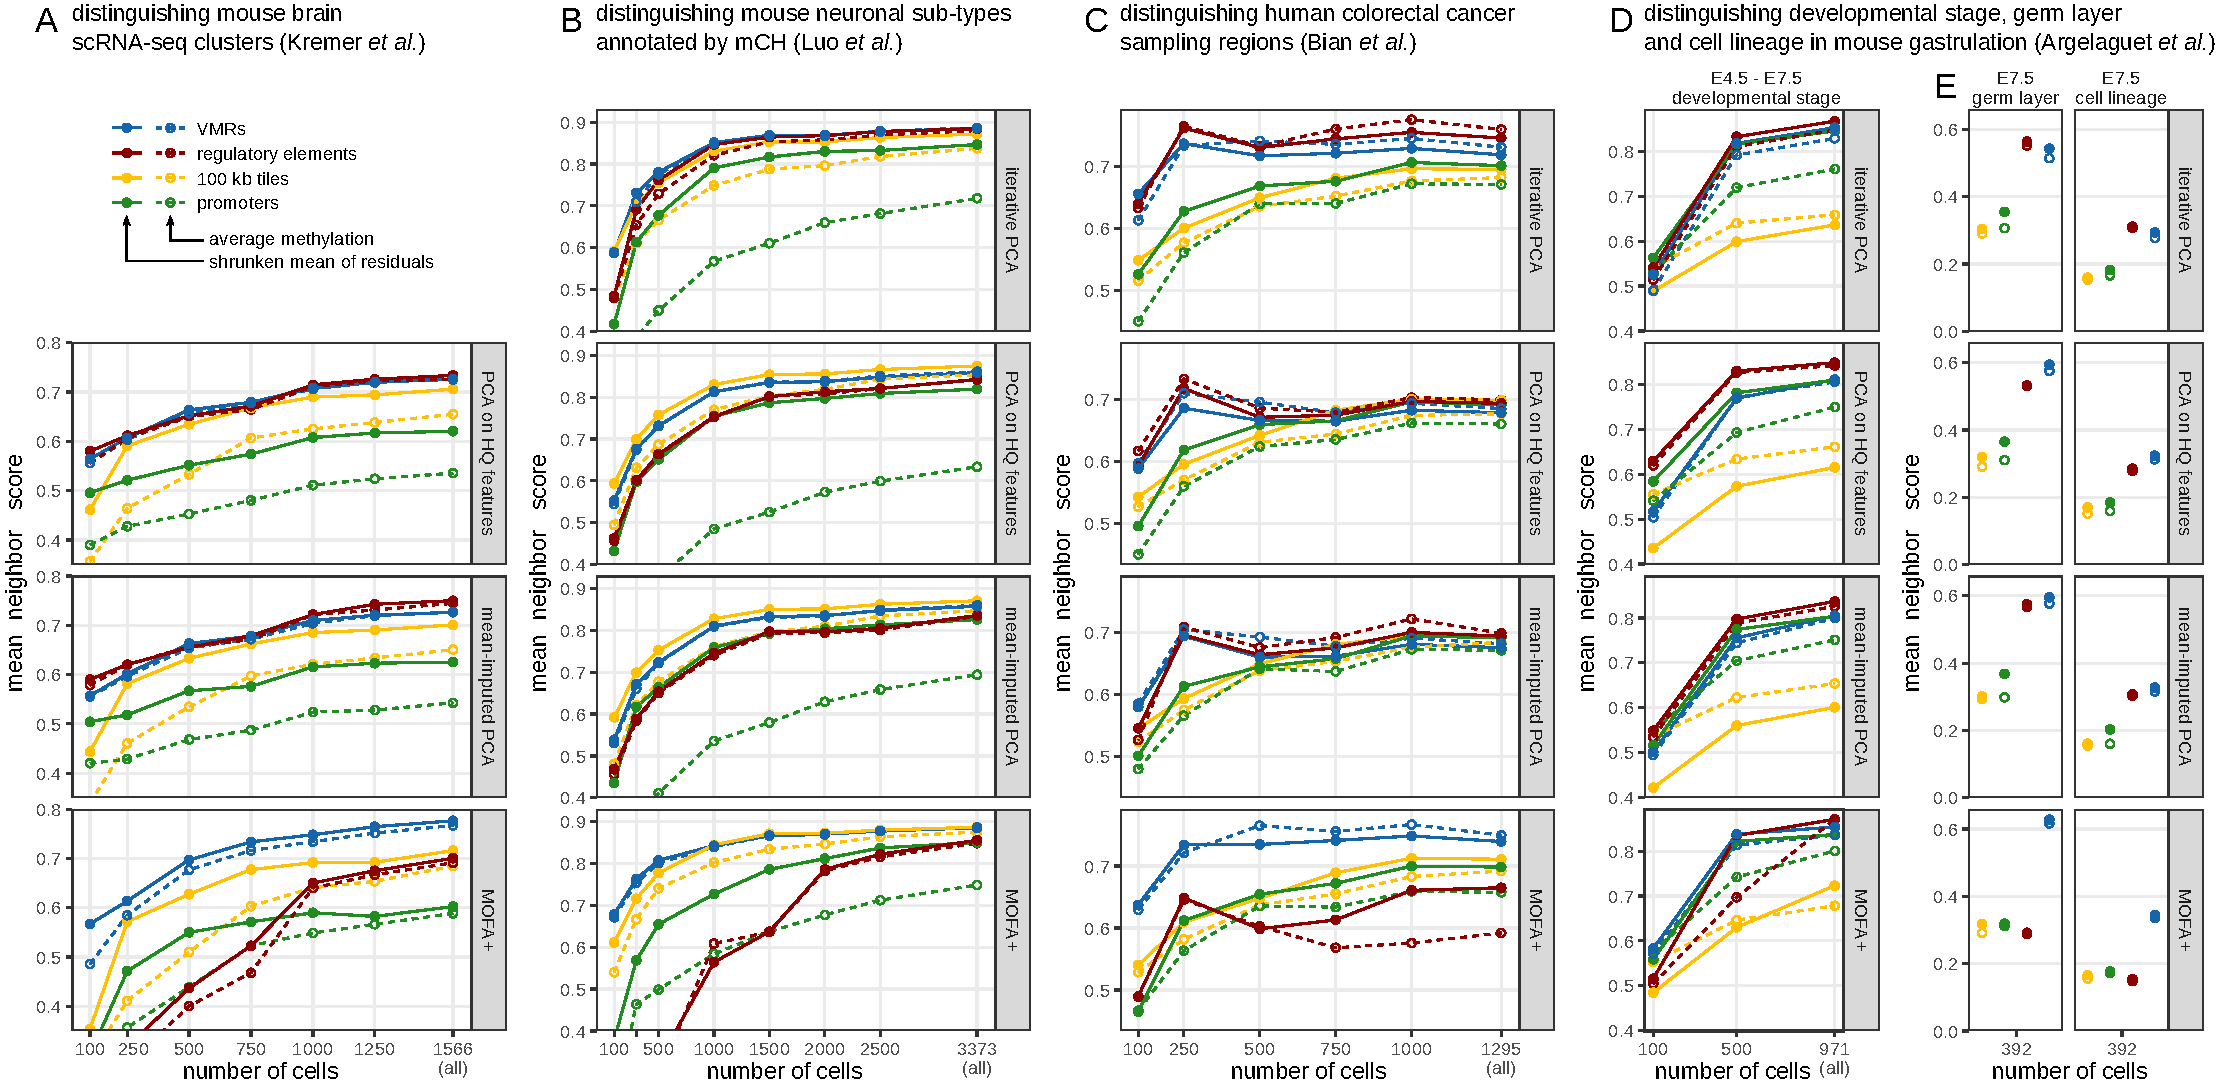
\includegraphics[width=\textwidth]{figures/SFig_benchmark.pdf}
	\end{center}
	\captionof{figure}{\small \textbf{Benchmark of several combinations of analysis methods on four single-cell methylation data sets.}\\
	\textbf{(A-E)} Benchmarking the ability to separate groups of cells based on CpG methylation data, using different analysis approaches.
	Methylation matrices were obtained either by averaging CpG methylation in genomic intervals (dotted lines, hollow points) or using the shrunken mean of residuals (solid lines and points).
	Each analysis was performed for the full data sets and sub-samples of each.
	Four sets of genomic intervals (VMRs, ENCODE regulatory elements, 100~kb tiles or promoters) were quantified and separately subjected to four dimensionality reduction techniques (see Methods for details):
	iterative PCA as proposed by us, mean-imputed PCA on intervals with high sequencing coverage \citep{luo2017single}, mean-imputed PCA on all intervals, and MOFA+ \citep{argelaguet2020mofa} on all intervals.
	For each combination of methods, we quantified the ability to use distance in 15-dimensional PCA space to separate ground-truth cell labels reported by the authors (neighbor score).
	\textbf{(A)} Separation of neural cell types/states annotated based on scRNA-seq of the same cells \citep{kremer_scnmt}.
	\textbf{(B)} Separation of neuron sub-types, annotated by averaging CH-methylation (mCH) in 100~kb genomic tiles \citep{luo2017single}.
	\textbf{(C)} Separation of human colorectal cancer sampling regions (primary tumor, normal adjacent tissue, lymph node metastasis, liver metastasis before and after treatment, omental metastasis) \citep{bian2018single}.
	\textbf{(D-E)} Separation of three properties of mouse embryo cells:
	The developmental stage (E4.5, E5.5, E6.5, E7.5), the germ layer or extra-embryonic tissue of origin, or the cell lineage.
	Germ layer and lineage (E, only E7.5-cells) were annotated by \citet{argelaguet2019gastru} based on scRNA-seq of the same cells.
	}
	\label{fig:score_luo}

\end{minipage}
\vfill
\newpage

\noindent%
\begin{minipage}{\linewidth}
    \begin{center}
        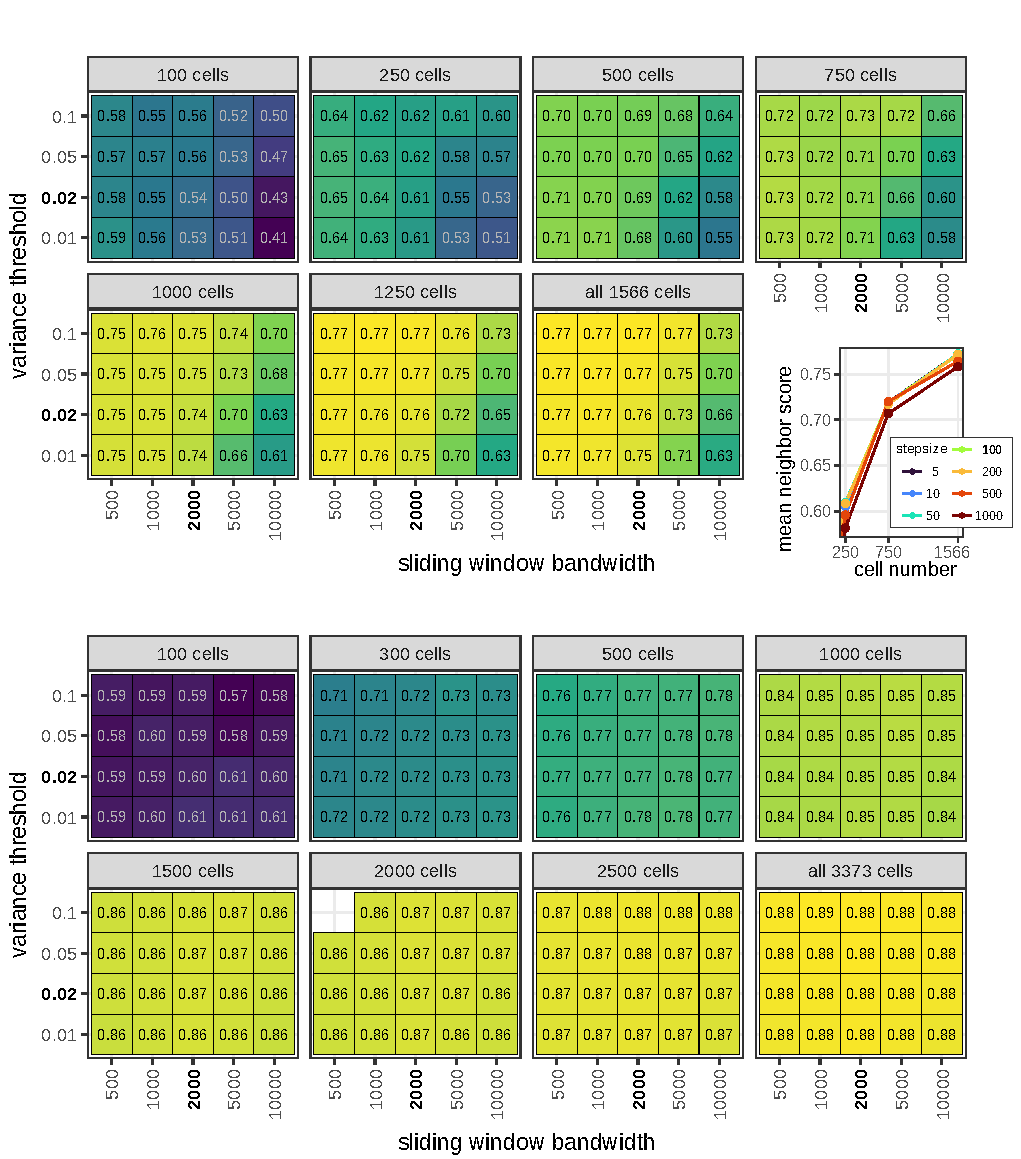
\includegraphics[width=.55\textwidth]{figures/SFig_parameter_sweep.pdf}
    \end{center}
    \captionof{figure}{\small \textbf{Effect of VMR detection parameters on separation of cell types.}\\
    \textbf{(A-B)} Mean neighbor scores obtained after analyzing single-cell methylomes from \citet{kremer_scnmt} (\textbf{A}) or \citet{luo2017single} (\textbf{B}) with our proposed methods.
    VMRs were detected with \texttt{methscan} \texttt{scan} using various sliding window bandwidths, variance thresholds, and on sub-samples of the full data sets.
    \textbf{(C)} Mean neighbor scores obtained after analyzing the \citet{kremer_scnmt} data set with various sliding window step sizes.
    }
    \label{fig:sweep}
\end{minipage}

\noindent%
\begin{minipage}{\linewidth}
	\begin{center}
		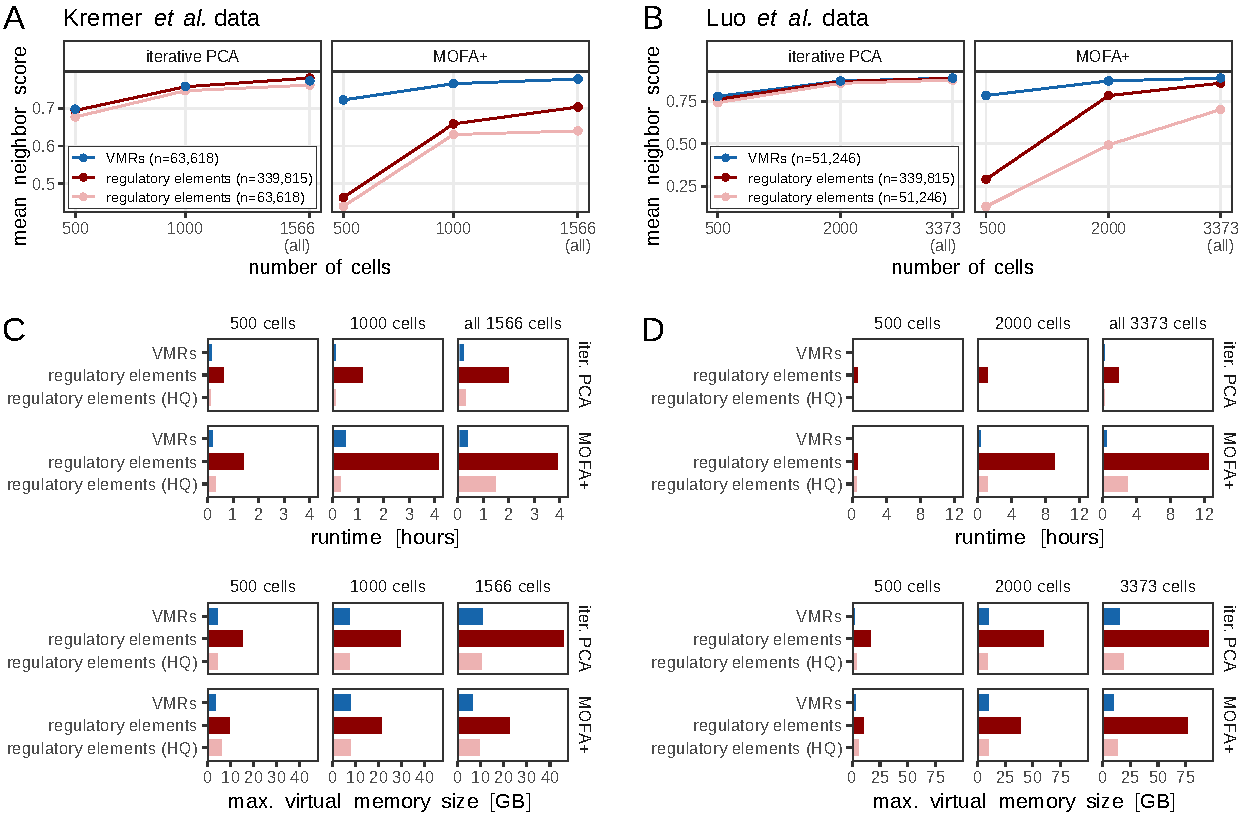
\includegraphics[width=.85\textwidth]{figures/SFig_benchmark_resources.pdf}
	\end{center}
	\captionof{figure}{\small \textbf{VMRs are more informative than an equal number of regulatory regions with high sequencing coverage.}\\
	\textbf{(A-B)} Mean neighbor score obtained when quantifying CpG methylation at VMRs, all ENCODE regulatory regions, or a subset of regulatory regions for the data sets of \citet{kremer_scnmt} and \citet{luo2017single}.
	The subset of high-quality (HQ) regulatory regions was selected in such a way that it matches the number of VMRs and contains those regulatory regions with the highest coverage.
	\textbf{(C-D)} Runtime (top) and RAM usage (bottom) of the two dimensionality reduction techniques shown in A and B.
	}
	\label{fig:resource_usage}
\end{minipage}

\noindent%
\begin{minipage}{\linewidth}
	\begin{center}
		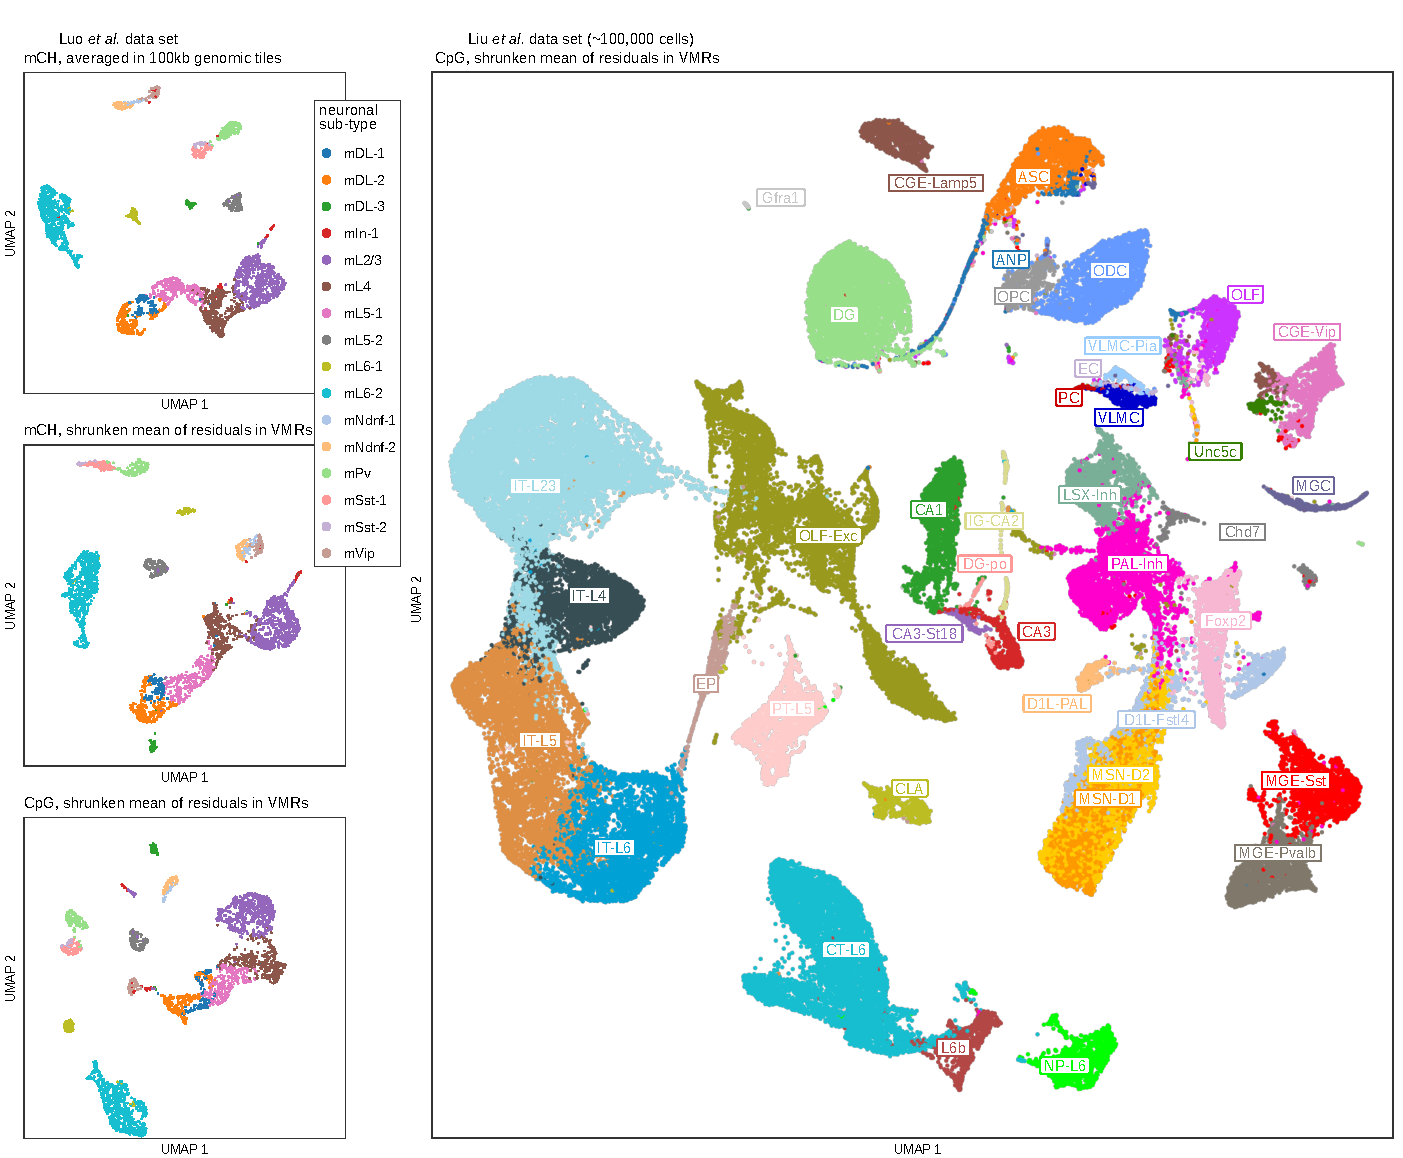
\includegraphics[width=.85\textwidth]{figures/SFig_100k_and_CH.pdf}
	\end{center}
	\captionof{figure}{\small \textbf{\textit{MethSCAn} performs well on CH-methylation data and on extremely large data sets.}\\
    \textbf{(A)} UMAPs obtained when analysing data from \citet{luo2017single} with three different strategies for producing a methylation matrix:
	top: averaging CH-methylation (mCH) in 100~kb genomic tiles (as done in \citep{luo2017single} to obtain the depicted cell type labels);
	center: using the shrunken mean of residuals to quantify mCH in mCH-VMRs;
	bottom: shrunken mean of residuals to quantify CpG methylation in CpG-VMRs.
	\textbf{(B)} UMAP obtained when analysing 100\,350 neural single-cell methylomes \citep{liu2021dna} with the default \textit{MethSCAn} workflow.
	The depicted cell labels were reported by \citet{liu2021dna}.
	Analysing this large data set takes approximately a week on a computer with 256 GB RAM and 48 CPUs, with almost all of this time (152 hours) spent by the \texttt{prepare} step, which is run only once per data set. The speed of this step can be increased considerably by processing chromosomes in parallel, which reduced the total runtime to approximately two days in our case.
	}
	\label{fig:umaps}
\end{minipage}

\end{document}
